% !TeX program = lualatex
% Compilacion recomendada: latexmk -lualatex plan_tesis_cables_pinn.tex
\RequirePackage{fix-cm}
\documentclass[11pt,a4paper,oneside]{report}

\usepackage{fontspec}
\setmainfont{Arial}
\setsansfont{Arial}
\newfontface\poppinsbold[Path=fonts/]{Poppins-Bold.ttf}
\usepackage[spanish,es-nodecimaldot,es-noshorthands]{babel}
\usepackage{csquotes}
\usepackage{geometry}
\geometry{
  a4paper,
  left=3cm,
  top=3cm,
  right=2.5cm,
  bottom=2.5cm,
  headheight=14pt,
  headsep=0.6cm
}
\usepackage{setspace}
\onehalfspacing
\usepackage{microtype}
\usepackage{graphicx}
\graphicspath{{imagenes/}}
\usepackage{booktabs}
\usepackage{longtable}
\usepackage{tabularx}
\usepackage{array}
\usepackage{multirow}
\usepackage{makecell}
\usepackage{threeparttable}
\usepackage{pdflscape}
\usepackage{ragged2e}
\usepackage{enumitem}
\usepackage{etoolbox}
\usepackage{titlesec}
\usepackage{fancyhdr}
\usepackage{amsmath,amssymb,mathtools}
\usepackage{siunitx}
\sisetup{output-decimal-marker={,},per-mode=symbol}
\usepackage{xcolor}
\usepackage{colortbl}
\definecolor{unired}{HTML}{8B1A1A}
\definecolor{darkblue}{HTML}{17365D}
\definecolor{lightblue}{HTML}{DCE6F1}
\definecolor{lightgray}{HTML}{F2F2F2}
\usepackage{tikz}
\usetikzlibrary{arrows.meta,positioning,shapes.geometric,fit,calc}
\usepackage{pgfplots}
\pgfplotsset{compat=1.18}
\usepackage{newfloat}
\usepackage{float}
\DeclareFloatingEnvironment[fileext=loe,listname={Listado de fórmulas},name=Fórmula,placement=htbp]{formula}
\DeclareFloatingEnvironment[fileext=lop,listname={Listado de procedimientos},name=Procedimiento,placement=htbp]{procedure}
\usepackage{caption}
\captionsetup{font=small,labelfont=bf,justification=centering}
\captionsetup[table]{font=footnotesize}
\AtBeginEnvironment{table}{\footnotesize}
\usepackage[hidelinks]{hyperref}
%\usepackage{xurl}

\hypersetup{
  pdftitle={Diseño y evaluación de un artefacto computacional basado en redes neuronales informadas por física para estimar la temperatura y la ampacidad de cables eléctricos enterrados en entornos térmicamente heterogéneos},
  pdfauthor={Luis Enrique Koc Góngora y Herbert Antonio Meléndez García},
  pdfsubject={Maestría en Inteligencia Artificial, Facultad de Ingeniería Industrial y de Sistemas, Universidad Nacional de Ingeniería}
}
\usepackage{bookmark}
\usepackage[backend=biber,style=apa,sortcites=true,sorting=nyt,maxcitenames=2,maxbibnames=20]{biblatex}
\DeclareLanguageMapping{spanish}{spanish-apa}
\DeclareFieldFormat{postnote}{#1}
\DeclareDelimFormat{postnotedelim}{\addcolon}
% Compatibilidad al leer listas auxiliares generadas con citas biblatex-apa.
\providecommand{\BLTXAPAifInParensTF}[3]{#3}
\addbibresource{referencias_plan_tesis.bib}
\setlength{\bibitemsep}{0.75\baselineskip}
\setlength{\bibparsep}{0pt}
% Incluir hasta cuarto nivel en el índice y numeración de secciones
\setcounter{tocdepth}{4}
% Numerar hasta el cuarto nivel de secciones (paragraph)
\setcounter{secnumdepth}{4}
\addto\captionsspanish{%
  \renewcommand{\listfigurename}{Listado de figuras}%
  \renewcommand{\listtablename}{Listado de tablas}%
  \renewcommand{\tablename}{Tabla}%
}

\newcommand{\tesisbodyfont}{\fontsize{11}{13.6}\selectfont}
\setlength{\parindent}{0pt}
% Equivale al espacio posterior de 12 pt de un procesador de textos y evita sangría inicial.
\setlength{\parskip}{12pt}
\setlength{\emergencystretch}{3em}
\setlist{
  leftmargin=1.1cm,
  before=\begin{spacing}{1}\tesisbodyfont,
  after=\end{spacing},
  topsep=.5\baselineskip,
  itemsep=.35\baselineskip,
  parsep=0pt,
  partopsep=0pt
}
\renewcommand{\arraystretch}{1.18}
\newcolumntype{Y}{>{%
  \RaggedRight
  \setlength{\parindent}{0pt}%
  \arraybackslash
}X}
\newcolumntype{J}{>{%
  \justifying
  \setlength{\parindent}{0pt}%
  \arraybackslash
}X}
\newcolumntype{L}[1]{>{%
  \RaggedRight
  \setlength{\parindent}{0pt}%
  \arraybackslash
}p{#1}}
\newcolumntype{C}[1]{>{%
  \Centering
  \setlength{\parindent}{0pt}%
  \arraybackslash
}p{#1}}

% El Anexo III prescribe Arial 11 para el cuerpo. Los niveles de titulo
% conservan ese tamaño y se distinguen mediante negrita y numeracion.
\titleformat{\chapter}[hang]
  {\normalfont\bfseries\fontsize{11}{13.2}\selectfont}
  {\MakeUppercase{\chaptername}\ \thechapter.}{0.75em}{\MakeUppercase}
\titleformat{name=\chapter,numberless}[block]
  {\normalfont\bfseries\fontsize{11}{13.2}\selectfont}
  {}{0pt}{\MakeUppercase}
\titlespacing*{\chapter}{0pt}{0pt}{0.75\baselineskip}
\titleformat{\section}
  {\normalfont\bfseries\fontsize{11}{13.2}\selectfont}
  {\thesection}{0.75em}{\MakeUppercase}
\titlespacing*{\section}{0pt}{1.0\baselineskip}{0.25\baselineskip}
\makeatletter
\newcommand*\tesis@tocnumberline[1]{#1.\enspace}
\renewcommand*\l@section[2]{%
  \begingroup
    \let\numberline\tesis@tocnumberline
    \@dottedtocline{1}{1.5em}{0pt}{#1}{#2}%
  \endgroup
}
\renewcommand*\l@subsection[2]{%
  \begingroup
    \let\numberline\tesis@tocnumberline
    \@dottedtocline{2}{3.8em}{0pt}{#1}{#2}%
  \endgroup
}
\renewcommand*\l@paragraph{\@dottedtocline{4}{8.8em}{3.0em}}
\makeatother
\titleformat{\subsection}
  {\normalfont\bfseries\fontsize{11}{13.2}\selectfont}
  {\thesubsection}{0.75em}{\MakeUppercase}
\titlespacing*{\subsection}{0pt}{0.75\baselineskip}{0.25\baselineskip}
\titleformat{\subsubsection}
  {\normalfont\bfseries\fontsize{11}{13.2}\selectfont}
  {\thesubsubsection}{0.75em}{\MakeUppercase}
\titlespacing*{\subsubsection}{0pt}{0.5\baselineskip}{0.25\baselineskip}

% Numeración: tres niveles numéricos y cuarto nivel con letras (a), b), ...)
\renewcommand\theparagraph{\alph{paragraph})}
\titleformat{\paragraph}
  {\normalfont\bfseries\fontsize{11}{13.2}\selectfont}
  {\theparagraph}{0.75em}{}
\titlespacing*{\paragraph}{0pt}{0.35\baselineskip}{0.2\baselineskip}

% Numeracion romana y arabiga en la esquina superior derecha.
\fancypagestyle{tesis}{
  \fancyhf{}
  \fancyhead[R]{\normalfont\fontsize{11}{13.2}\selectfont\thepage}
  \renewcommand{\headrulewidth}{0pt}
  \renewcommand{\footrulewidth}{0pt}
}
\fancypagestyle{plain}{
  \fancyhf{}
  \fancyhead[R]{\normalfont\fontsize{11}{13.2}\selectfont\thepage}
  \renewcommand{\headrulewidth}{0pt}
  \renewcommand{\footrulewidth}{0pt}
}
\pagestyle{tesis}

\newcommand{\Tmax}{T_{\max}}
\newcommand{\Imax}{I_{\max}}
\newcommand{\kx}{k(x,y)}
\newcommand{\pct}{\mbox{\char37}}
\newcommand{\tituloTesis}{Diseño y evaluación de un artefacto computacional basado en redes neuronales informadas por física para estimar la temperatura y la ampacidad de cables eléctricos enterrados en entornos térmicamente heterogéneos}

\begin{document}
\hypersetup{pageanchor=false}

% ---------------------------------------------------------------------------
% CARATULA: Guia N. 01, ejemplo para maestria de especializacion.
% ---------------------------------------------------------------------------
\begin{titlepage}
\thispagestyle{empty}
\begin{singlespace}
\setlength{\parskip}{0pt}
\begin{center}
{\poppinsbold\fontsize{22}{26.4}\selectfont
\makebox[\textwidth][c]{UNIVERSIDAD NACIONAL DE INGENIERÍA}\par}
\vspace{0.55cm}
{\fontsize{16}{19.2}\selectfont\bfseries UNIDAD DE POSGRADO DE LA FACULTAD DE INGENIERÍA INDUSTRIAL Y DE SISTEMAS\par}
{\fontsize{16}{19.2}\selectfont\bfseries ESCUELA DE POSGRADO\par}

\vspace{0.4cm}

\includegraphics[width=7.5cm]{logo_UNI.png}

\vspace{0.4cm}
{\fontsize{14}{16.8}\selectfont\bfseries PLAN DE TESIS\par}
\vspace{0.25cm}
{\fontsize{14}{16.8}\selectfont\bfseries\MakeUppercase{\tituloTesis}\par}

\vfill
{\fontsize{12}{14.4}\selectfont
PARA OBTENER EL GRADO ACADÉMICO DE\par
MAESTRO CON MENCIÓN EN:\par
INTELIGENCIA ARTIFICIAL\par}

\vspace{0.6cm}
{\fontsize{12}{14.4}\selectfont\bfseries ELABORADA POR:\par}
\vspace{0.2cm}
{\fontsize{12}{14.4}\selectfont\bfseries LUIS ENRIQUE KOC GÓNGORA\par}
{\fontsize{12}{14.4}\selectfont\bfseries HERBERT ANTONIO MELÉNDEZ GARCÍA\par}

\vspace{0.55cm}
{\fontsize{12}{14.4}\selectfont\bfseries ASESOR: SAMUEL OPORTO\par}

\vfill
{\fontsize{14}{16.8}\selectfont\bfseries LIMA, PERÚ\par}
\vspace{0.15cm}
{\fontsize{12}{14.4}\selectfont\bfseries 2026\par}
\end{center}
\end{singlespace}
\end{titlepage}

\tesisbodyfont
\hypersetup{pageanchor=true}
\pagenumbering{roman}
\setcounter{page}{2}

\chapter*{DATOS GENERALES}
\addcontentsline{toc}{chapter}{DATOS GENERALES}
\vspace{0.35cm}

\begingroup
\singlespacing
\setlength{\parskip}{0pt}
\setlength{\parindent}{0pt}
\setlength{\tabcolsep}{10pt}
\renewcommand{\arraystretch}{1.28}
\noindent
\begin{tabularx}{\textwidth}{
  >{\bfseries\RaggedRight\setlength{\parindent}{0pt}\arraybackslash}p{4.15cm}
  J
}
\toprule
\rowcolor{lightgray}
\textbf{Elemento} & \textbf{Descripción} \\
\midrule
Título del plan & \tituloTesis. \\
\addlinespace[5pt]
Tesistas & \mbox{Luis Enrique Koc Góngora};\newline
           \mbox{Herbert Antonio Meléndez García}. \\
\addlinespace[5pt]
Programa & Maestría en Inteligencia Artificial. \\
\addlinespace[5pt]
Unidad académica & Unidad de Posgrado de la Facultad de Ingeniería Industrial y de Sistemas, Universidad Nacional de Ingeniería. \\
\addlinespace[5pt]
Área involucrada & Inteligencia artificial científica, modelado computacional y sistemas eléctricos de potencia. \\
\addlinespace[5pt]
Lugar de desarrollo & Entorno computacional de la Facultad de Ingeniería Industrial y de Sistemas de la Universidad Nacional de Ingeniería (FIIS-UNI) y casos de referencia documentados de instalaciones de cables eléctricos subterráneos. \\
\addlinespace[5pt]
Duración estimada & Doce meses, desde julio de 2026 hasta junio de 2027. \\
\addlinespace[5pt]
Tipo de graduación & Maestría de especialización o profesionalizante. \\
\addlinespace[5pt]
Artefacto de\newline investigación & Modelo y prototipo computacional 2D basado en redes neuronales informadas por física para analizar campos térmicos y ampacidad en entornos heterogéneos. \\
\bottomrule
\end{tabularx}
\endgroup

% \chapter*{Resumen}
% \addcontentsline{toc}{chapter}{Resumen ejecutivo}
% \justifying
% El desempeño de un cable eléctrico subterráneo está limitado por la temperatura alcanzada por su conductor, la cual depende de las pérdidas internas y de la capacidad del entorno para evacuar calor. Los métodos normativos de ampacidad son indispensables como referencia de ingeniería, pero representan el terreno mediante resistencias térmicas equivalentes y supuestos simplificados; en campo, la humedad, el secado, los estratos, el \textit{bedding} y el \textit{backfill} producen una conductividad térmica espacialmente variable. Esta diferencia puede ocultar puntos calientes o inducir estimaciones conservadoras de capacidad \parencites[4--6]{enescu2021}[41--42]{cigre2025}.

% La investigación propone diseñar y evaluar, bajo el paradigma de ciencia del diseño (DSR), un artefacto computacional que incorpore la ecuación de conducción de calor, las condiciones de contorno e interfaz y la conductividad térmica espacialmente variable $\kx$ dentro del entrenamiento de una red neuronal informada por física (PINN). El artefacto será demostrado en casos analíticos, benchmarks FEM y escenarios documentados de cables enterrados; su evaluación considerará exactitud térmica, conservación de energía, robustez, costo computacional y capacidad para estimar la ampacidad. La secuencia metodológica adapta las actividades de identificación del problema, objetivos de solución, diseño, demostración, evaluación y comunicación de DSRM, con ciclos formativos de refinamiento durante el desarrollo \parencites[55--56]{peffers2007}[200--202]{delport2024}.

% Se espera producir un modelo lógico, un prototipo reproducible, un conjunto de escenarios y principios de diseño transferibles a la clase de problemas de conducción térmica 2D multimaterial. La contribución no se reducirá al software: incluirá criterios de representación de heterogeneidad, procedimientos de verificación y evidencia sobre cuándo la aproximación homogénea puede sesgar la temperatura máxima o la corriente admisible \parencites[343--350]{gregor2013}[93--99]{cigre2025}.

% \noindent\textbf{Palabras clave:} cable subterráneo; ampacidad; heterogeneidad térmica; conductividad del suelo; red neuronal informada por física; ciencia del diseño.

\begingroup
\singlespacing
\tesisbodyfont
\tableofcontents
\listoffigures
\listoftables
\listofformulas
\listofprocedures
\endgroup

\clearpage
\pagenumbering{arabic}

% ===========================================================================
\chapter{PLANTEAMIENTO DEL PROBLEMA}
\thispagestyle{empty}

Este capítulo establece el hilo conductor del plan de tesis. Primero presenta el sistema cable--instalación--entorno térmico; luego delimita la brecha entre un entorno heterogéneo y su representación homogénea. Esa brecha permite formular el problema de investigación.

\section{INTRODUCCIÓN}

En los sistemas eléctricos, los cables subterráneos permiten transportar energía cuando existen restricciones de espacio, seguridad, servidumbre o integración con otras infraestructuras \parencite{cigre2020tb815}. Su capacidad de transporte no depende únicamente del conductor, sino del sistema cable--instalación--entorno térmico y de la forma en que este conjunto disipa el calor. Comprender esa relación es necesario para aprovechar la infraestructura instalada sin comprometer la temperatura admisible, la confiabilidad ni la vida útil de los cables \parencites[1--3]{enescu2020}[41--42]{cigre2025}.

Durante la operación, un cable conduce corriente eléctrica y disipa hacia el entorno el calor generado, principalmente, debido a las pérdidas por efecto Joule. En este estudio, la ampacidad \(\Imax\) se entiende como la máxima corriente que puede circular sin que el conductor supere su temperatura admisible \parencites[752]{neher1957}[1]{enescu2020}. Por tanto, su estimación requiere considerar tanto el diseño del cable como las condiciones térmicas de la instalación.

En instalaciones enterradas, el entorno incluye el arreglo de cables, los rellenos de mejora térmica, la zanja y el suelo nativo \parencites{enescu2021}{ieee442}{kim2025}. La humedad, los estratos del suelo, los rellenos y las interfaces entre materiales hacen que ese entorno sea térmicamente heterogéneo y modifican la disipación del calor y la temperatura máxima del conductor \(\Tmax\) \parencites[1,6--7]{khumalo2025}[1--3]{aldulaimi2024}. Una representación que no capture esas variaciones puede sobreestimar la capacidad térmica y elevar el riesgo durante la operación; una aproximación demasiado conservadora puede, en cambio, dejar capacidad instalada sin utilizar \parencite[41--42]{cigre2025}.

Los métodos normalizados para calcular la ampacidad representan el sistema mediante redes de resistencias térmicas y propiedades equivalentes \parencites[752--760]{neher1957}{iec60287}{iec60853}. Esta simplificación facilita el cálculo, pero puede ocultar variaciones relevantes del campo de temperatura \(T(x,y)\) cuando la conductividad térmica \(\kx\) cambia espacialmente \parencites[41--42]{cigre2025}[1--3]{aldulaimi2024}. Los métodos numéricos, como el método de elementos finitos (FEM), permiten describir el terreno con mayor detalle, aunque requieren preparar el dominio, la discretización y cada escenario de cálculo \parencites[93--99]{cigre2025}[1--3,12]{aldulaimi2024}.

La problemática central surge de la diferencia entre el entorno térmico heterogéneo de una instalación enterrada y su representación simplificada en el cálculo de la ampacidad. Para examinar esta brecha, se necesita una forma verificable de representar la conductividad térmica \(\kx\), estimar el campo de temperaturas \(T(x,y)\) y cuantificar en qué medida la heterogeneidad térmica modifica \(\Tmax\) e \(\Imax\). Esta necesidad vincula el problema físico con la búsqueda de una alternativa computacional que pueda evaluarse frente a referencias conocidas.

Para abordar la brecha, el estudio construirá un artefacto computacional abierto y verificable basado en una red neuronal informada por física (PINN). En este enfoque, la ecuación de conducción de calor y las condiciones de frontera e interfaz se incorporan al proceso de entrenamiento para aproximar el campo térmico \parencite{raissi2019}. Sin embargo, no se asumirá que la PINN constituye una mejora automática, porque la convergencia, los pesos de pérdida, las interfaces y el costo de entrenamiento pueden condicionar su desempeño \parencites[1--2,14--17]{lawal2022}[2--6]{ren2025}.

El estudio seguirá el paradigma de la ciencia del diseño (DSR), de acuerdo con la secuencia metodológica de \textcite[55--56]{peffers2007}. Este enfoque permitirá construir el artefacto y evaluar su utilidad dentro del sistema cable--instalación--entorno térmico. La evaluación comparará sus resultados con casos analíticos, referencias FEM y escenarios documentados, conforme a los criterios de construcción y evaluación de artefactos propuestos por \textcite[342--344]{gregor2013}.

En conjunto, la investigación busca determinar si un artefacto PINN puede representar la heterogeneidad térmica con suficiente trazabilidad para apoyar la estimación de \(T(x,y)\), \(\Tmax\) e \(\Imax\). La sección siguiente sitúa esta necesidad dentro de las exigencias actuales de las redes eléctricas y del uso de instalaciones subterráneas.

\section{PROBLEMÁTICA}

Las redes eléctricas atraviesan una etapa de mayor exigencia operativa porque la generación, la demanda y la participación renovable siguen aumentando. En América Latina y el Caribe, la generación eléctrica creció 5,5\,\pct{} en 2024 y la renovabilidad regional alcanzó 69\,\pct{}; además, la energía solar llegó a 7\,\pct{} de la matriz \parencite{olade2025generacionALC2024}. En el Perú, la producción eléctrica nacional creció a una tasa media anual de 2,4\,\pct{} entre 2023 y 2025, mientras que la máxima demanda del SEIN aumentó 2,2\,\pct{} anual en el mismo periodo; estas tasas son cálculo propio a partir de las cifras originales de MINEM y COES \parencites{minem2025anuario2024}{minem2025indicadoresDiciembre}{coesMaximaDemanda}.

La presión sobre la red no proviene solo del crecimiento total, sino también del cambio en la matriz. En el Perú, la participación conjunta de la producción solar y eólica en la generación nacional pasó de un valor cercano a cero en 2010 a 5,3\,\pct{} en 2023, 8,1\,\pct{} en 2024 y 9,5\,\pct{} en 2025. Estos porcentajes son cálculos propios a partir de la serie anual de producción por origen del MINEM; el valor de 2025 se basa en cifras preliminares \parencites[sec.~10.4]{minem2025anuario2024}[cuadro~4]{minem2025indicadoresDiciembre}. Esta tendencia es consistente con el diagnóstico del COES, que considera proyectos eólicos y solares entre las opciones de nueva generación eficiente para el SEIN \parencite[18--20]{coes2023diagnostico2025_2034}, y con la advertencia de la IEA sobre la necesidad de que la red avance al ritmo de la expansión renovable \parencite{iea2025transmissiongrid}.

La Figura~\ref{fig:participacion-renovable-peru} muestra el aumento de la participación conjunta de esas dos fuentes. El indicador no mide por sí mismo congestión ni sobrecarga de la red; su función es mostrar el cambio de contexto que incrementa la necesidad de planificar conexiones y utilizar con criterio la capacidad de transporte disponible.

\begin{figure}[htbp]
\centering
\begin{tikzpicture}
\begin{axis}[
  width=0.88\textwidth,
  height=0.46\textwidth,
  ylabel={Participación en la generación nacional (\pct{})},
  xlabel={Año},
  xmin=2009.5, xmax=2025.5,
  xtick={2010,2012,2014,2016,2018,2020,2022,2024,2025},
  xticklabel={\pgfmathprintnumber[fixed,precision=0,1000 sep={}]{\tick}},
  xticklabel style={rotate=45,anchor=east,font=\footnotesize},
  ymin=0, ymax=11,
  ytick={0,2,4,6,8,10},
  grid=major,
  grid style={gray!25},
  axis line style={black!70},
  tick label style={font=\footnotesize},
  label style={font=\footnotesize}
]
\addplot[color=darkblue,mark=*,mark size=2.2pt,very thick] coordinates {
  (2010,0.003)
  (2011,0.003)
  (2012,0.138)
  (2013,0.457)
  (2014,1.003)
  (2015,1.711)
  (2016,2.524)
  (2017,2.582)
  (2018,4.095)
  (2019,4.245)
  (2020,4.915)
  (2021,4.572)
  (2022,4.610)
  (2023,5.336)
  (2024,8.124)
  (2025,9.510)
};
\end{axis}
\end{tikzpicture}
\caption[Participación de la generación solar y eólica en el Perú]{Participación conjunta de la generación solar y eólica en la producción eléctrica nacional del Perú, 2010--2025. Fuente: Elaboración propia con datos del Ministerio de Energía y Minas \parencites[sec.~10.4]{minem2025anuario2024}[cuadro~4]{minem2025indicadoresDiciembre}. Nota: el valor de 2025 corresponde a cifras preliminares.}
\label{fig:participacion-renovable-peru}
\end{figure}

La serie muestra una incorporación gradual hasta 2023 y una aceleración durante 2024--2025. En esos dos últimos años, la participación conjunta aumentó 4,2 puntos porcentuales respecto de 2023 y fue aproximadamente 1,8 veces el valor de ese año. Este crecimiento no demuestra que todos los tramos de la red estén sometidos al mismo nivel de exigencia; sí respalda la necesidad general de acompañar la nueva generación con infraestructura y métodos de evaluación que permitan conocer los márgenes de operación.

En este contexto, los cables subterráneos se vuelven más relevantes en tramos donde las redes enfrentan restricciones de espacio, servidumbre, seguridad, integración urbana, cruces o conexión de instalaciones \parencite{cigre2020tb815}. Sin embargo, su uso eficiente exige estimar con cuidado la ampacidad, porque la capacidad disponible depende del balance térmico con el entorno enterrado y de sus condiciones reales \parencites{fariz2026}{mobius2025}.

La dificultad técnica surge porque la capacidad de un cable subterráneo no depende solo de su sección o de su aislamiento. También depende de la forma en que el calor generado se disipa hacia el suelo, los rellenos y las capas constructivas que rodean la instalación. Los métodos clásicos y las normas de cálculo son necesarios como base de ingeniería, pero suelen representar el entorno mediante resistencias térmicas equivalentes para hacer tratable el cálculo \parencites[752--760]{neher1957}{iec60287}{iec60853}.

Esa representación puede ser débil cuando el terreno real no se comporta como un medio homogéneo. La humedad, los estratos, el \textit{bedding}, el \textit{backfill}, la profundidad y las zonas secas pueden modificar la conductividad térmica alrededor del cable \parencites[4--6]{enescu2021}[1--3]{aldulaimi2024}. En consecuencia, dos instalaciones con la misma corriente pueden alcanzar temperaturas distintas si el entorno enterrado ofrece caminos térmicos diferentes.

La evidencia muestra que el estado del suelo puede modificar de forma sustancial la capacidad de transporte. \textcite[5--6, tabs.~2--3]{khumalo2025} midieron una resistividad térmica de \SI{0.596}{\kelvin\metre\per\watt} con 14,5\,\pct{} de humedad y de \SI{3.72}{\kelvin\metre\per\watt} en estado seco. Para esos extremos, la ampacidad media calculada disminuyó de \SI{518.34}{\ampere} a \SI{224.21}{\ampere}. Además, cuando combinaron suelo seco, una profundidad de \SI{1150}{\milli\metre} y una temperatura del suelo de \SI{28}{\celsius}, obtuvieron una reducción superior a 45\,\pct{} respecto de las condiciones ideales.

La Figura~\ref{fig:resistividad-ampacidad-khumalo} representa los cinco pares publicados de resistividad térmica y ampacidad media. La serie permite observar la magnitud y la dirección de la relación sin reducirla a la comparación de sus dos valores extremos.

\begin{figure}[htbp]
\centering
\begin{tikzpicture}
\begin{axis}[
  width=0.84\textwidth,
  height=0.48\textwidth,
  xlabel={Resistividad térmica del suelo (\si{\kelvin\metre\per\watt})},
  ylabel={Ampacidad media (\si{\ampere})},
  xmin=0.4, xmax=3.9,
  ymin=180, ymax=550,
  xtick={0.596,1.2,1.646,2.341,3.72},
  xticklabels={{0,596},{1,200},{1,646},{2,341},{3,720}},
  ytick={200,250,300,350,400,450,500,550},
  grid=major,
  grid style={gray!25},
  axis line style={black!70},
  tick label style={font=\footnotesize},
  label style={font=\footnotesize},
  line width=0.9pt
]
\addplot[color=darkblue,mark=*,mark size=2.5pt,very thick] coordinates {
  (0.596,518.34)
  (1.2,382.13)
  (1.646,330.47)
  (2.341,280.01)
  (3.72,224.21)
};
\end{axis}
\end{tikzpicture}
\caption[Relación entre resistividad térmica del suelo y ampacidad]{Relación entre resistividad térmica del suelo y ampacidad media calculada para tres cables. Fuente: Elaboración propia con datos de \textcite[5--6, tabs.~2--3]{khumalo2025}.}
\label{fig:resistividad-ampacidad-khumalo}
\end{figure}

La tendencia descendente de la Figura~\ref{fig:resistividad-ampacidad-khumalo} indica que la ampacidad calculada no permanece constante cuando cambia la condición térmica del suelo. Entre los extremos reportados, la reducción es de aproximadamente 56,7\,\pct{}. Este resultado no se generaliza como una tasa universal, porque corresponde a los cables y supuestos analizados por los autores; sin embargo, evidencia por qué la caracterización espacial del entorno puede ser relevante para una estimación térmica trazable.

Los materiales de relleno también modifican la respuesta térmica de la instalación. \textcite[1,10,16]{kim2025} reportan un agregado de concreto premezclado con conductividad de \SI{2.094}{\watt\per\metre\per\kelvin}, frente a \SI{1.365}{\watt\per\metre\per\kelvin} de la arena natural. Bajo condiciones críticas, ese cambio redujo la temperatura máxima de \SI{77.6}{\celsius} a \SI{70.6}{\celsius}. Por tanto, el relleno no es un detalle constructivo menor, sino una condición que puede cambiar la capacidad térmica disponible.

La dificultad también es operativa porque las propiedades del suelo y de los rellenos no se observan directamente a lo largo de toda una instalación durante el servicio. Por ello, la estimación de capacidad debe combinar supuestos documentados, datos del sitio y modelos térmicos cuya respuesta pueda verificarse. Las revisiones recientes sobre clasificación térmica de cables subterráneos destacan precisamente la dependencia de la ampacidad respecto del entorno, las condiciones de frontera y la calidad del modelo utilizado \parencites{fariz2026}{mobius2025}.

La tensión metodológica aparece al decidir cómo representar ese entorno en el cálculo. Un modelo homogéneo es rápido y útil para diseño preliminar, pero puede ocultar zonas locales de baja disipación térmica. Un modelo FEM puede representar con mayor detalle la geometría y las propiedades espaciales, aunque exige construir, mallar, verificar y repetir escenarios \parencites[3--4,93--99]{cigre2025}[1--3]{aldulaimi2024}. Por ello, la dificultad del proyecto se concentra en cuantificar, con trazabilidad, cómo la heterogeneidad térmica cambia $\Tmax$ e $\Imax$ frente a una representación homogénea equivalente.

La Figura~\ref{fig:brecha} sintetiza la relación entre presión de red, uso de cables subterráneos, entorno térmico heterogéneo, simplificación homogénea y riesgo de decisión. La dificultad central es que una diferencia no cuantificada en $\Tmax$ o $\Imax$ puede afectar tanto la seguridad del suministro como el uso eficiente de la capacidad de red.

Si el modelo subestima la temperatura, puede permitir una corriente excesiva. En consecuencia, puede acelerar el envejecimiento del cable o producir fallas prematuras \parencite[1--2,9]{khumalo2025}. En cambio, si el modelo sobreestima la temperatura, puede limitar capacidad disponible sin necesidad. Por ello, también puede favorecer decisiones de sobredimensionamiento \parencites[4--6]{enescu2021}[1--2,9]{khumalo2025}.

\vspace{0.15cm}

\begin{figure}[htbp]
\centering
\resizebox{1.0\textwidth}{!}{%
\begin{tikzpicture}[
  scale=1.,
  transform shape,
  box/.style={draw,rounded corners=3pt,align=center,text width=3.25cm,minimum height=1.25cm,font=\tiny},
  arr/.style={-{Stealth[length=3mm]},thick},
  darr/.style={-{Stealth[length=3mm]},thick,dashed}]
\node[box,fill=lightgray] (cables) {Tramos con cables\\subterráneos\\restricciones de espacio,\\servidumbre y seguridad};
\node[box,fill=lightblue,right=0.75cm of cables] (real) {Entorno térmico\\enterrado\\$\kx$ variable: humedad,\\estratos, secado, \textit{backfill}};
\node[box,fill=red!10,right=0.75cm of real] (gap) {Diferencia no\\cuantificada\\$\Delta \Tmax$ y $\Delta \Imax$};
\node[box,fill=yellow!15,below=1.0cm of cables] (context) {Presión de red\\SEIN, demanda, renovables\\continuidad y capacidad};
\node[box,fill=green!10,below=1.0cm of real] (simpl) {Representación\\homogénea\\$k=k_{eq}$ y resistencias\\térmicas equivalentes};
\node[box,fill=orange!12,below=1.0cm of gap] (impact) {Riesgo de decisión\\subestimar: envejecimiento\\sobreestimar: capacidad ociosa};
\draw[arr] (context) -- (cables);
\draw[arr] (cables) -- (real);
\draw[arr] (real) -- (gap);
\draw[arr] (real) -- (simpl);
\draw[arr] (simpl) -- (gap);
\draw[darr] (context.south) -- ($(context.south)+(0,-0.55cm)$)
  -- ($(impact.south)+(0,-0.55cm)$) -- (impact.south);
\draw[arr] (gap) -- (impact);
\draw[arr] (simpl) -- (impact);
\end{tikzpicture}
}%
\caption{Relación entre presión de red, uso de cables subterráneos, entorno térmico heterogéneo, simplificación homogénea y riesgo de decisión. Fuente: Elaboración propia.}
\label{fig:brecha}
\end{figure}

En síntesis, la problemática del proyecto se ubica en redes que requieren mayor capacidad, continuidad y conexión de nueva generación, mientras algunos tramos subterráneos dependen de condiciones térmicas enterradas difíciles de observar. Si esas condiciones se simplifican en exceso, la estimación de temperatura y ampacidad puede orientar decisiones inseguras o conservadoras. Esta situación conduce al planteamiento del problema de investigación.

%\section{IDENTIFICACIÓN Y DESCRIPCIÓN ABSTRACTA DEL PROBLEMA DE ESTUDIO}

\section{PLANTEAMIENTO DEL PROBLEMA}
\label{sec:planteamiento-problema}

En términos generales, este es un problema de transferencia de calor. Se aplica a sistemas multimateriales con propiedades térmicas que cambian en el espacio. Dada una geometría, fuentes de calor, condiciones de frontera e interfaces, se requiere aproximar $T(x,y)$. A partir de ese campo, se obtienen $\Tmax$ e $\Imax$.

Sin embargo, el problema no se resuelve con un promedio simple de propiedades, porque la geometría, las interfaces y las discontinuidades del suelo interactúan entre sí. Por tanto, la brecha es metodológica y de análisis: existen cálculos normativos y modelos FEM detallados, pero falta una formulación integrada, reproducible y verificada \parencites{iec60287}{iec60853}[3--4,93--99]{cigre2025}. Esa formulación debe mostrar cómo la heterogeneidad térmica modifica la temperatura máxima y la ampacidad. Además, debe evitar que cada escenario dependa solo de rehacer modelos FEM con mayor costo computacional.

El objeto de estudio es el sistema cable--instalación--entorno térmico en cables subterráneos. Este sistema reúne el cable multicapa, la instalación, el \textit{bedding}, el \textit{backfill}, el suelo nativo y las condiciones de operación \parencites[3--6]{enescu2021}{ieee442}[1,10]{kim2025}. La unidad de análisis será una sección transversal 2D de una instalación con cable XLPE. Además, incluirá suelo nativo, relleno de zanja y, cuando corresponda, relleno con propiedades térmicas mejoradas.

El interés no recae en una marca específica de cable. En cambio, se centra en configuraciones representativas y reproducibles, tanto en disposición plana como en trébol. Por tanto, el artefacto PINN 2D será el producto tecnológico usado para estudiar el sistema. No será el objeto físico de estudio.

\subsection{FORMULACIÓN DEL PROBLEMA}

La formulación se presenta a continuación y se organiza en la matriz de consistencia del ANEXO 5.1, la cual funciona como un organizador lógico del plan. Por tanto, la matriz relaciona problema, objetivos, hipótesis, variables, evidencia y controles, además de evitar que las partes del estudio queden como ideas separadas. Los problemas específicos siguen la lógica DSR. Por ello, delimitan entradas del problema, productos verificables y criterios de evaluación del artefacto.

\subsubsection{PROBLEMA GENERAL}

Existen técnicas para estimar temperatura y ampacidad en cables subterráneos, pero los casos con entorno térmico heterogéneo mantienen una limitación práctica \parencites[4--6]{enescu2021}[3--4,93--99]{cigre2025}. Las representaciones homogéneas equivalentes son rápidas, aunque no describen de forma explícita la conductividad variable $\kx$. En cambio, los modelos FEM sí la representan, pero exigen construir, mallar y verificar cada escenario. Por tanto, resulta difícil cuantificar de forma reproducible cómo la heterogeneidad modifica $T(x,y)$, $\Tmax$ e $\Imax$.

\subsubsection{PROBLEMAS ESPECÍFICOS}

\begin{enumerate}[label=PE\arabic*.]
  \item No está formalizado qué información debe ingresar al artefacto. Por tanto, falta ordenar cable multicapa, interfaces, fuentes, contornos y $\kx$ en escenarios heterogéneos.
  \item No se dispone de un paquete reproducible de referencias analíticas, manufacturadas, FEM y casos publicados. Sin ese paquete, la verificación previa queda débil.
  \item No existe una evaluación trazable de escenarios controlados de contraste, extensión y proximidad. Debido a ello, no se conoce con claridad el cambio en $\Tmax$, $T(x,y)$ y punto caliente.
  \item No están identificadas las condiciones que producen la mayor discrepancia de ampacidad. La comparación debe hacerse entre una representación homogénea y una representación 2D heterogénea verificada.
  \item No se ha sistematizado un procedimiento reproducible a partir de la evidencia del artefacto. Además, faltan principios transferibles para problemas 2D multimateriales.
\end{enumerate}

\subsection{JUSTIFICACIÓN}

\subsubsection{JUSTIFICACIÓN PRÁCTICA}

La investigación permitirá identificar configuraciones donde un valor homogéneo puede ocultar una restricción térmica local. Esta posibilidad se relaciona con los cambios de capacidad por humedad y resistividad reportados por \textcite[1,6--9]{khumalo2025}.

Además, el estudio puede apoyar decisiones de diseño, verificación y operación. Esto aplica cuando la evacuación de energía depende de circuitos enterrados con bajo margen térmico \parencite[14842,14851]{fariz2026}.

\subsubsection{JUSTIFICACIÓN TECNOLÓGICA}

El artefacto combinará conocimiento físico y aprendizaje automático para producir un campo térmico diferenciable, ya que incorporará la PDE en la función de pérdida durante el entrenamiento \parencite[686--690]{raissi2019}. Además, buscará reducir la dependencia exclusiva de pares etiquetados generados por FEM, la cual aparece en enfoques híbridos recientes para cables \parencite[1--3,12]{aldulaimi2024}.

Sin embargo, la propuesta no pretende reemplazar a FEM ni a las normas IEC. En cambio, busca establecer cuándo una PINN es suficientemente exacta y qué costos presenta \parencite[93--99]{cigre2025}.

\subsubsection{JUSTIFICACIÓN METODOLÓGICA}

El enfoque DSR vincula el problema físico con la construcción y evaluación del artefacto \parencite[55--56]{peffers2007}. Por tanto, el estudio no se limita a ejecutar software, sino que aportará un procedimiento reproducible de especificación y verificación. También propondrá principios de diseño sobre interfaces y heterogeneidad del terreno. Este énfasis sigue la distinción entre artefacto situado y contribución abstracta de \textcite[342--350]{gregor2013}.

\subsubsection{JUSTIFICACIÓN CIENTÍFICA Y ACADÉMICA}

El trabajo conectará dos cuerpos de conocimiento: el dimensionamiento térmico de cables enterrados y el aprendizaje informado por física. Esta conexión permite llevar las PINN a un problema aplicado de ingeniería.

Los resultados de PINN en dominios térmicos controlados ya han sido reportados \parencites[1--3,17]{xing2023}[1,3,16]{pan2025}. Sin embargo, aquí se evaluarán en una geometría multimaterial, donde el entrenamiento y las interfaces todavía deben verificarse \parencite[2--6]{ren2025}.

\section{ALCANCES Y LIMITACIONES}

\subsection{ALCANCES}

\begin{itemize}[itemsep=0.60\baselineskip, topsep=0.35\baselineskip]
  \item \textbf{Temático:} conducción de calor en secciones 2D de cables XLPE enterrados, con heterogeneidad de suelo, \textit{bedding} y \textit{backfill}; cálculo de temperatura y ampacidad.
  \item \textbf{Metodológico:} diseño y evaluación de un artefacto basado en redes PINN bajo la metodología DSR, comparado con referencias analíticas, soluciones basadas en FEM y casos publicados.
  \item \textbf{Espacial:} configuraciones representativas de circuitos eléctricos formados por cables enterrados para la evacuación de energía eléctrica en centrales solares y eólicas; no se restringe a una única instalación propietaria.
  \item \textbf{Temporal:} desarrollo previsto entre julio de 2026 y junio de 2027; la revisión bibliográfica tendrá como fecha de corte junio de 2026.
  \item \textbf{Producto:} arquitectura lógica, prototipo de red PINN, datos de escenarios, pruebas, informe de evaluación y principios de diseño reproducibles.
\end{itemize}

\subsection{LIMITACIONES}

El estudio será principalmente estacionario y bidimensional. El régimen transitorio se limitará a pruebas seleccionadas, debido a que la capacidad dinámica aún presenta retos de convergencia e incertidumbre \parencite[14851--14852]{fariz2026}.

El modelo no resolverá la interacción electromagnética completa del cable. Por tanto, las pérdidas eléctricas se representarán como una fuente de calor por efecto Joule, proporcional a $I^2R$ \parencites[752--760]{neher1957}[cláusulas 4--5]{iec60287}.

Tampoco se modelarán envejecimiento dieléctrico, humedad acoplada, migración de humedad ni convección subterránea. En consecuencia, las propiedades del suelo, \textit{bedding} y \textit{backfill} se tratarán como entradas por escenario.

La evaluación del artefacto se limitará a verificación y comparación documentada. Por verificación se entenderá la comparación con casos analíticos, soluciones manufacturadas, referencias FEM y casos publicados \parencites{cigre2022}[3--4,93--99]{cigre2025}.

No se realizará validación experimental de campo, debido a que requeriría instrumentación y seguimiento de una instalación real. Por tanto, los resultados no se generalizarán fuera de las geometrías, materiales, fuentes y contornos evaluados.

Además, cualquier ventaja computacional se reportará junto con hardware, tolerancias, semillas e inicializaciones. Así se comunicará la evidencia con límites claros, como exige la metodología DSR \parencite[350--351]{gregor2013}.

% ===========================================================================
\chapter{OBJETIVOS DE LA INVESTIGACIÓN}
\thispagestyle{empty}

Este capítulo convierte el problema formulado en objetivos, hipótesis y dimensiones operativas. Así, mantiene la continuidad entre la brecha técnica y las decisiones metodológicas del estudio.

La secuencia parte del objetivo general, continúa con objetivos específicos y termina en factores, resultados y controles. Por ello, la matriz de consistencia puede leerse como el organizador lógico del plan.

\section{OBJETIVOS}

\subsection{OBJETIVO GENERAL}

Diseñar y evaluar un artefacto computacional basado en una red neuronal informada por física (PINN). El artefacto estudiará el sistema cable--instalación--entorno térmico en cables subterráneos, estimará $T(x,y)$, $\Tmax$ e $\Imax$, y permitirá cuantificar el efecto de la heterogeneidad térmica espacial del entorno.

\subsection{OBJETIVOS ESPECÍFICOS}

\begin{enumerate}[label=OE\arabic*.]
  \item Especificar las entradas físicas, requisitos funcionales y criterios de calidad del artefacto para representar el sistema cable--instalación--entorno térmico, incluyendo dominios multicapa, fuentes térmicas, condiciones de contorno, interfaces y conductividad térmica espacialmente variable $\kx$.
  \item Construir y verificar el artefacto usando como insumos soluciones analíticas o manufacturadas, benchmarks FEM con convergencia y casos publicados.
  \item Evaluar escenarios controlados de contraste, patrón, extensión y proximidad de heterogeneidades del suelo y los rellenos para obtener cambios en $\Tmax$, el campo de temperatura $T(x,y)$ y la localización del punto caliente.
  \item Comparar la ampacidad obtenida con representación 2D heterogénea frente a escenarios homogéneos equivalentes e identificar las condiciones de entrada que generan mayor discrepancia.
  \item Formular, a partir de los resultados del artefacto, principios de diseño y un procedimiento reproducible para aplicar y evaluar PINN en problemas térmicos multimateriales de cables enterrados.
\end{enumerate}

\section{HIPÓTESIS}

\subsection{HIPÓTESIS GENERAL}

La incorporación explícita de $\kx$ en un artefacto PINN 2D permitirá reproducir referencias verificadas. Además, mostrará diferencias de temperatura máxima y ampacidad frente a un entorno homogéneo equivalente cuando existan regiones de baja o alta conductividad próximas al cable. Por tanto, el proceso deberá reportar trazabilidad y costo computacional.

\subsection{HIPÓTESIS ESPECÍFICAS}

\begin{enumerate}[label=HE\arabic*.]
  \item Una especificación que separe PDE, contornos, interfaces, fuentes y propiedades térmicas reducirá ambigüedades. Además, permitirá definir pruebas de consistencia física y funcional.
  \item El artefacto alcanzará, en el dominio de verificación, error relativo de $\Tmax$ no mayor a 5\,\pct{}. Además, tendrá NRMSE no mayor a 5\,\pct{} y desequilibrio energético no mayor a 2\,\pct{}.
  \item A igualdad de geometría, pérdidas y contornos, una región de baja $k$ cercana al conductor aumentará $\Tmax$. En cambio, una región de alta $k$ usada como relleno reducirá $\Tmax$.
  \item La aproximación homogénea tenderá a sobreestimar $\Imax$ cuando promedie una zona local de baja $k$. Por tanto, la discrepancia crecerá con el contraste y la extensión.
  \item Los principios extraídos del artefacto serán aplicables a problemas 2D multimateriales. Sin embargo, esa aplicación requiere trazabilidad, pruebas, límites de validez y métricas de calidad.
\end{enumerate}

Los umbrales de HE2 son criterios de aceptación del proyecto, no valores universales de PINN. Se revisarán en la fase piloto para que la incertidumbre numérica sea menor que el efecto térmico analizado, según la verificación de herramientas de ampacidad señalada por \textcite[93--99]{cigre2025}. Además, cualquier ajuste deberá reportar límites de validez con evidencia suficiente, como recomiendan \textcite[350--351]{gregor2013} para contribuciones DSR.

\section{DIMENSIONES OPERATIVAS DEL ESTUDIO}
\label{sec:dimensiones-operativas}

En coherencia con la metodología DSR, las dimensiones operativas ordenan el objeto de estudio y la evaluación del artefacto. Por tanto, no se presentan como pares estadísticos aislados.

Primero, la matriz de consistencia organiza la relación entre problema, objetivos, hipótesis, evidencia y controles. Luego, la matriz de operacionalización convierte esa relación en variables observables.

Las variables independientes se tratarán como \textit{factores} de configuración física y numérica. El factor principal será la conductividad térmica espacialmente variable $\kx$, cuyos niveles se expresarán mediante contraste, patrón, extensión y proximidad al conductor. Debido a ello, $\kx$ representa suelo nativo, \textit{bedding}, \textit{backfill}, humedad o secado.

La matriz de operacionalización de variables del \ref{anx:operacionalizacion-variables} lleva esta lectura a un plano práctico. Allí se muestra qué se modifica, qué se calcula, qué se registra y qué condiciones se conservan.

\subsection{VARIABLES INDEPENDIENTES (FACTORES)}

Los factores independientes son entradas que se modificarán de manera controlada. Entre ellos están la representación de conductividad, el contraste $C_k$, el patrón, la extensión, la proximidad y la referencia.

Sin embargo, la geometría, las pérdidas y los contornos se mantendrán constantes en cada comparación pareada. Así será posible atribuir los cambios observados a $\kx$.

\subsection{VARIABLES DEPENDIENTES (RESULTADOS)}

Las variables dependientes son los resultados que entrega el artefacto. Incluyen $T(x,y)$, $\Tmax$, punto caliente, $\Imax$, diferencia de ampacidad y métricas de error. Por tanto, no se interpretarán como simples salidas de software, sino como evidencia para aceptar, ajustar o limitar el artefacto dentro del ciclo DSR.

\subsection{DISEÑO EXPERIMENTAL FACTORIAL}

El diseño experimental será factorial en sentido metodológico, porque combinará niveles de contraste, patrón, extensión y proximidad para observar efectos sobre $\Tmax$ e $\Imax$. Sin embargo, no se aplicará análisis factorial estadístico para reducir variables latentes, sino un diseño factorial de escenarios numéricos, desarrollado en el \ref{anx:diseno-factorial}.

La Tabla~\ref{tab:dimensiones-operativas} resume esa organización y separa sistema físico, factores, respuestas, calidad del artefacto y controles. Con base en esa clasificación, la Figura~\ref{fig:modelo-conceptual} muestra el encadenamiento del análisis: primero, $\kx$ modifica el campo térmico; luego, ese campo determina el límite operativo.

Por tanto, los controles se mantienen explícitos. Así, las diferencias observadas pueden atribuirse al entorno térmico y no a cambios de geometría, pérdidas o condiciones numéricas.

\begin{figure}[H]
\centering
\resizebox{0.9\textwidth}{!}{%
\begin{tikzpicture}[
  var/.style={draw,rounded corners=3pt,align=center,text width=3.5cm,minimum height=1.2cm,font=\small},
  arr/.style={-{Stealth[length=3mm]},thick}]
\node[var,fill=lightblue] (x) {Factor independiente\\conductividad térmica $\kx$\\$C_k$, patrón, extensión, proximidad};
\node[var,fill=green!12,right=1.5cm of x] (t) {Resultado térmico\\campo de temperatura $T(x,y)$\\$\Tmax$, punto caliente};
\node[var,fill=orange!15,right=1.5cm of t] (i) {Resultado operativo\\$\Imax$, margen y discrepancia};
\node[var,fill=lightgray,below=1.3cm of t] (c) {Controles\\geometría, pérdidas, contornos y configuración numérica};
\draw[arr] (x) -- (t);
\draw[arr] (t) -- (i);
\draw[arr,dashed] (c) -- (x);
\draw[arr,dashed] (c) -- (t);
\draw[arr,dashed] (c) -- (i);
\end{tikzpicture}
}%
\caption{Modelo conceptual de las relaciones evaluadas. Fuente: Elaboración propia.}
\label{fig:modelo-conceptual}
\end{figure}

\begin{table}[H]
\centering
\caption{Dimensiones operativas, factores y resultados de la investigación.}
\label{tab:dimensiones-operativas}
\begingroup
\scriptsize
\setlength{\tabcolsep}{3pt}
\renewcommand{\arraystretch}{1.42}
\begin{tabularx}{\textwidth}{L{3.0cm}L{2.75cm}Y Y}
\toprule
\textbf{Dimensión} & \textbf{Papel metodológico} & \textbf{Definición conceptual} & \textbf{Componentes o indicadores} \\
\midrule
Sistema cable--instalación--entorno térmico & Sistema estudiado y objeto de estudio & Unidad física en la que se genera, conduce y disipa calor desde el conductor hacia el entorno. & Cable XLPE multicapa; disposición plana o trébol; \textit{bedding}; \textit{backfill}; suelo nativo; profundidad; condiciones térmicas de operación. \\
Sección transversal 2D del sistema & Unidad de análisis & Caso computacional donde se representa la geometría, materiales, fuentes, contornos y referencia de comparación. & Dominio $\Omega$; región del conductor $\Omega_c$; interfaces; caso analítico, manufacturado, FEM o publicado. \\
Conductividad térmica espacialmente variable del entorno, $\kx$ & Variable independiente: factor físico principal & Variación espacial de la capacidad conductora del suelo, asiento y relleno. & Magnitud; contraste $C_k$; patrón; extensión; proximidad; tipo de material o estado hídrico. \\
Configuración factorial de la heterogeneidad & Variables independientes: niveles del factor & Combinación controlada de los niveles usados para producir escenarios comparables. & Contraste bajo/medio/alto; proximidad cercana/media/lejana; extensión pequeña/media/grande; patrón estratificado, localizado, relleno o zona seca. \\
Temperatura del conductor & Variable dependiente: resultado térmico & Respuesta térmica del cable ante pérdidas y transferencia de calor al entorno. & $\Tmax$; temperatura media; $\Delta\Tmax$; campo de temperatura $T(x,y)$; gradiente; ubicación del punto caliente. \\
Ampacidad & Variable dependiente: resultado operativo & Corriente máxima compatible con el límite térmico del conductor. & $\Imax$; variación porcentual; \textit{derating}/\textit{uprating}; margen térmico. \\
Exactitud y calidad del artefacto & Resultado de evaluación DSR & Grado en que el artefacto es válido, útil, reproducible y eficiente. & Error; residuos; balance de energía; robustez entre semillas; tiempo y memoria; cobertura de requisitos. \\
Geometría, pérdidas y contornos & Variables controladas & Condiciones que deben permanecer constantes en comparaciones pareadas. & Diámetros; profundidad; separación; corriente; pérdidas; temperatura ambiente; tamaño del dominio y condiciones de borde. \\
Variabilidad numérica y documental & Variables no controladas registradas & Condiciones que pueden afectar la comparación y que se documentarán para no ocultar incertidumbre. & Semilla; convergencia; tolerancia FEM publicada; disponibilidad de datos; incertidumbre de propiedades; hardware y versión del código. \\
\bottomrule
\end{tabularx}
\endgroup
\end{table}


% ===========================================================================
\chapter{METODOLOGÍA DE LA INVESTIGACIÓN}
\label{ch:metodologia}
\thispagestyle{empty}

Este capítulo explica cómo se evaluará la respuesta planteada en los objetivos. Para mantener la concordancia con el problema, la metodología conserva como eje la relación entre $\kx$, $T(x,y)$, $\Tmax$ e $\Imax$.

La ciencia del diseño organiza ese proceso porque el estudio construye un artefacto y lo evalúa con evidencia. Por tanto, cada fase metodológica produce una salida verificable.

\section{METODOLOGÍA}
\label{sec:metodologia}

La investigación tendrá enfoque cuantitativo porque calculará y comparará temperatura, errores, residuos, tiempos y variaciones de ampacidad. Además, esos registros se obtendrán mediante casos analíticos, manufacturados, bibliográficos y computacionales del sistema cable--instalación--entorno térmico.

Será aplicada y tecnológica porque construirá un artefacto para estudiar un problema de ingeniería. Por tanto, evaluará tanto el efecto de $\kx$ como la utilidad del artefacto.

Como maestría de especialización, el diseño metodológico se organizará como ciencia del diseño. Primero se especificará el problema; luego se construirá el artefacto; finalmente se demostrará, evaluará y comunicará.

La metodología seguirá el paradigma DSR porque el estudio debe demostrar que el artefacto funciona y que su diseño produce conocimiento transferible. La estructura de identificación, diseño, demostración, verificación y comunicación se toma de \textcite[55--56]{peffers2007}; dentro de esa secuencia se contrastarán proposiciones sobre $\kx$, $\Tmax$ e $\Imax$. Las métricas cuantitativas serán evidencia del ciclo DSR, de acuerdo con el énfasis de \textcite[349--351]{gregor2013} en utilidad, calidad, eficacia y comunicación de la contribución. Por esta razón, la metodología distingue objeto físico, entradas, configuración, producto, evidencia y controles, en lugar de tratar las dimensiones operativas como pares estadísticos aislados \parencites[55--56]{peffers2007}[342--344]{gregor2013}.

\subsection{ADAPTACIÓN DE LA CIENCIA DEL DISEÑO}

El Procedimiento~\ref{proc:dsr} resume cómo se adaptan las actividades DSR al estudio y muestra la función de cada una dentro del ciclo de construcción, demostración, evaluación y comunicación del artefacto.

\begin{procedure}[htbp]
\caption{Proceso DSR adaptado al estudio.}
\label{proc:dsr}
\begin{enumerate}[label=\textbf{A\arabic*.}]
  \item \textbf{Identificación y motivación:} delimitar el sistema cable--instalación--entorno térmico, la clase de problema, las entradas físicas relevantes y la diferencia operativa entre $k_{eq}$ y la conductividad térmica espacialmente variable $\kx$.
  \item \textbf{Objetivos de solución:} convertir problemas y requisitos físicos en productos verificables, criterios cuantificables de exactitud, robustez, utilidad y reproducibilidad.
  \item \textbf{Diseño y desarrollo:} definir la arquitectura lógica del artefacto, la representación computacional del sistema físico, sus entradas y salidas esperadas, implementar incrementos y registrar decisiones y versiones.
  \item \textbf{Demostración:} ejecutar referencias, benchmarks y escenarios de heterogeneidad representativos para mostrar los resultados que produce el artefacto.
  \item \textbf{Evaluación:} comparar productos y resultados con los criterios de aceptación, analizar errores y decidir refinamiento o aceptación.
  \item \textbf{Comunicación:} documentar artefacto, insumos, resultados, evidencia, límites, principios de diseño y productos académicos.
\end{enumerate}
\end{procedure}

La secuencia seguirá a \textcite[55--56]{peffers2007}; sin embargo, la evaluación también será formativa. Por tanto, cada incremento deberá superar pruebas físicas y numéricas antes de usarse en la demostración. Esta decisión adopta el refinamiento continuo recomendado por \textcite[198--203]{delport2024}.

\subsection{ARTEFACTO PROPUESTO}

El artefacto será un modelo y prototipo computacional, por lo que no se reducirá a una red entrenada. A nivel lógico tendrá seis componentes, mostrados en la Figura~\ref{fig:arquitectura}. La especificación evitará decisiones prematuras sobre bibliotecas, hardware o clases de software, ya que esas decisiones se tomarán después de confirmar requisitos. Además, se registrarán como parte de la búsqueda de diseño.

\begin{figure}[htbp]
\centering
\begin{tikzpicture}[
  comp/.style={draw,rounded corners=3pt,align=center,text width=3.6cm,minimum height=1.25cm,font=\small},
  arr/.style={-{Stealth[length=2.8mm]},thick}]
\node[comp,fill=lightblue] (spec) {1. Especificación del caso\\geometría, materiales, carga y contornos};
\node[comp,fill=lightblue,right=1.0cm of spec] (phys) {2. Representación física\\PDE, fuentes, interfaces\\y conductividad variable $\kx$};
\node[comp,fill=green!12,right=1.0cm of phys] (solver) {3. Solucionador PINN\\aproximación y entrenamiento};
\node[comp,fill=orange!12,below=1.15cm of solver] (eval) {4. Verificación y evaluación\\referencias, residuos, balance y robustez};
\node[comp,fill=orange!12,left=1.0cm of eval] (exp) {5. Experimentación numérica\\casos, sensibilidad y ampacidad};
\node[comp,fill=lightgray,left=1.0cm of exp] (report) {6. Trazabilidad\\datos, metadatos, resultados e informes};
\draw[arr] (spec) -- (phys);
\draw[arr] (phys) -- (solver);
\draw[arr] (solver) -- (eval);
\draw[arr] (eval) -- (exp);
\draw[arr] (exp) -- (report);
\draw[arr,dashed] (eval.north) to[bend left=25] (phys.south);
\draw[arr,dashed] (report.north) to[bend left=25] (spec.south);
\end{tikzpicture}
\caption{Arquitectura lógica del artefacto DSR propuesto. Fuente: Elaboración propia.}
\label{fig:arquitectura}
\end{figure}

Los componentes expresan el artefacto a un nivel lógico, de modo que separan los principios de diseño de una implementación particular. Esta separación favorece la reutilización y responde a la recomendación de \textcite[342--350]{gregor2013} sobre describir artefacto, requisitos y búsqueda de diseño. El mismo esquema recoge la evaluación continua recomendada por \textcite[198--203]{delport2024}.

\subsection{MODELO FÍSICO}
\label{subsec:modelo-fisico}

Para régimen estacionario, la temperatura se gobernará por la conservación de energía en un medio de conductividad espacialmente variable. Esta forma se toma de la ecuación clásica de conducción de calor para medios heterogéneos y se adapta al dominio 2D del estudio \parencites{carslaw1959conduction,kakac2018heatConduction,hahn2012heatConduction}[3]{xing2023}:

\begin{formula}
\centering
\begin{equation}
\label{for:calor}
\nabla\!\cdot\!\left(\kx\nabla T(x,y)\right)+Q(x,y)=0,
\qquad (x,y)\in\Omega .
\end{equation}
\caption{Ecuación de conducción de calor 2D estacionaria.}
\end{formula}

La Fórmula~\ref{for:calor} expresa el balance estacionario usado como núcleo físico del artefacto. En ella, $Q$ representa las pérdidas volumétricas o una distribución equivalente de fuentes, mientras que $\kx$ mantiene la variación de material dentro del operador térmico. Por ello, la formulación evita tratar las discontinuidades como cambios externos al operador y es coherente con PINN que incluyen propiedades espaciales \parencite[3]{xing2023}.

En las interfaces se impondrá continuidad de temperatura y de flujo normal. En el contorno se usarán condiciones de temperatura, flujo o convección, según el caso de referencia \parencite[3--5]{enescu2020}.

\begin{formula}
\centering
\begin{equation}
\label{for:interfaz}
T_1=T_2,
\qquad
\mathbf{n}\cdot k_1\nabla T_1=\mathbf{n}\cdot k_2\nabla T_2
\quad \text{en }\Gamma_{12}.
\end{equation}
\caption{Condiciones de interfaz entre dos materiales.}
\end{formula}

La Fórmula~\ref{for:interfaz} hace explícita esa restricción: la temperatura debe ser continua y el flujo normal debe conservarse entre materiales. Esta condición proviene del balance térmico en interfaces y es relevante porque el dominio incluye cable, relleno y suelo, de modo que las interfaces no pueden introducir saltos térmicos sin justificación física \parencites{carslaw1959conduction,kakac2018heatConduction}{patankar1980numerical}[3]{xing2023}.

La PINN aproximará el campo $T_\theta(x,y)$ y minimizará una pérdida compuesta, la cual incluirá residuos de ecuación, contornos, interfaces y datos de referencia cuando existan \parencite[686--690]{raissi2019}. Este esquema sigue la penalización física propuesta por \textcite[686--690]{raissi2019}; sin embargo, los pesos no se fijarán de antemano. Los pesos serán parte de la búsqueda de diseño, debido a que gradientes desbalanceados pueden sesgar la convergencia en redes PINN \parencites[16]{pan2025}[1--2,17]{lawal2022}.

\begin{formula}
\centering
\begin{equation}
\label{for:loss}
\mathcal{L}(\theta)=
w_f\mathcal{L}_{\mathrm{PDE}}+
w_b\mathcal{L}_{\mathrm{cont}}+
w_i\mathcal{L}_{\mathrm{int}}+
w_d\mathcal{L}_{\mathrm{datos}}+
w_e\mathcal{L}_{\mathrm{energía}}.
\end{equation}
\caption{Función de pérdida lógica del artefacto PINN.}
\end{formula}

La Fórmula~\ref{for:loss} organiza el entrenamiento como una suma ponderada de restricciones. Es una formulación operacional del estudio basada en la pérdida PINN de \textcite[686--690]{raissi2019} y en los problemas de ponderación reportados por \textcite[1--2,17]{lawal2022} y \textcite[16]{pan2025}. El término $\mathcal{L}_{\mathrm{PDE}}$ penaliza el incumplimiento de la ecuación de calor; los términos de contorno e interfaz controlan condiciones físicas auxiliares; los datos y la energía agregan trazabilidad cuando exista una referencia.

La ampacidad se obtendrá buscando la corriente que hace coincidir $\Tmax$ con el límite térmico adoptado. Este criterio se basa en la definición clásica de corriente admisible y en el tratamiento normativo de régimen permanente para cables \parencites[752--760]{neher1957}[cláusulas 4--5]{iec60287}[3--6]{enescu2021}. En cada iteración se actualizarán las pérdidas dependientes de corriente y luego se resolverá el campo térmico hasta cumplir tolerancias de temperatura y energía.

\begin{formula}
\centering
\begin{equation}
\label{for:ampacidad}
\Imax=\max\left\{I:\max_{(x,y)\in\Omega_c}T(x,y;I)\leq T_{\mathrm{lim}}\right\}.
\end{equation}
\caption{Condición para calcular la ampacidad.}
\end{formula}

La Fórmula~\ref{for:ampacidad} convierte ese criterio en una condición operacional para el artefacto. La corriente admisible es el mayor valor de $I$ que mantiene la temperatura máxima del conductor, evaluada en $\Omega_c$, por debajo del límite térmico $T_{\mathrm{lim}}$. Por tanto, el cálculo de ampacidad depende directamente de la calidad del campo $T(x,y;I)$.

\subsection{CONTEXTO DE APLICACIÓN Y UNIDAD DE ANÁLISIS}
\label{subsec:unidad-analisis}

Por tratarse de una maestría de especialización, la unidad de análisis no será una población estadística, sino una sección transversal 2D del sistema cable--instalación--entorno térmico. Cada caso se definirá por entradas físicas y computacionales, entre ellas geometría, disposición, propiedades térmicas, carga, contornos, referencia de comparación y versión del artefacto. Los valores de cables, materiales y entorno térmico se tomarán de fuentes bibliográficas, normas, casos publicados, soluciones analíticas o supuestos declarados. El artefacto PINN será la unidad de intervención. Por tanto, su evaluación seguirá la lógica DSR.

Los casos se seleccionarán por pertinencia técnica y capacidad de evaluación. Se usarán soluciones analíticas, soluciones manufacturadas, benchmarks FEM, configuraciones publicadas y escenarios representativos. Así, los casos mostrarán alcance, límites y utilidad del artefacto. Sin embargo, no se levantarán mediciones directas de campo ni se buscará inferencia probabilística sobre todas las instalaciones posibles.

\subsection{EXPERIMENTACIÓN NUMÉRICA DEL ARTEFACTO DENTRO DE DSR}

La experimentación numérica permitirá observar el comportamiento térmico del sistema y servirá para demostrar y evaluar el artefacto dentro de la metodología DSR. No se planteará como un diseño experimental autónomo orientado a inferencia estadística, sino como una secuencia de casos controlados. Primero, la secuencia verificará el prototipo con casos simples y trazables; luego, demostrará su uso en configuraciones con $\kx$. Finalmente, evaluará la diferencia entre representaciones heterogéneas y homogéneas equivalentes para estimar el efecto sobre $\Tmax$ e $\Imax$.

Las comparaciones serán pareadas y controladas. Por tanto, cuando se evalúe heterogeneidad, solo cambiará la representación térmica del entorno. Además, los barridos de contraste, extensión y proximidad mostrarán sensibilidad física y límites del artefacto. La Tabla~\ref{tab:experimentacion-dsr} ordena esa secuencia dentro del ciclo DSR.

\begin{table}[htbp]
\centering
\caption{Uso de la experimentación numérica dentro del ciclo DSR.}
\label{tab:experimentacion-dsr}
\begin{tabularx}{\textwidth}{L{3.2cm}Y Y}
\toprule
\textbf{Momento DSR} & \textbf{Propósito de la experimentación numérica} & \textbf{Evidencia esperada} \\
\midrule
Verificación formativa & Comprobar que las entradas físicas, PDE, contornos, interfaces, pérdidas y cálculo de ampacidad están implementados de forma coherente. & Paquete de pruebas, errores frente a casos analíticos/manufacturados, residuos, balance de energía y correcciones registradas. \\
Demostración & Mostrar que el artefacto puede transformar escenarios de cable subterráneo con materiales heterogéneos en campos térmicos interpretables. & Mapas del campo de temperatura $T(x,y)$, $\Tmax$, punto caliente, trazabilidad de entrada--salida y comparación con referencias FEM o publicadas. \\
Evaluación DSR & Juzgar utilidad, robustez, reproducibilidad y límites frente a escenarios homogéneos equivalentes. & Diferencias de $\Tmax$ y ampacidad, métricas de robustez, criterios de aceptación y principios de diseño derivados. \\
\bottomrule
\end{tabularx}
\end{table}

\subsection{EVIDENCIA, INSTRUMENTOS Y TRAZABILIDAD}

La evidencia provendrá de revisión documental, casos analíticos o manufacturados, referencias FEM, configuraciones publicadas y ejecuciones computacionales registradas. Por tanto, cada fuente deberá quedar asociada a un uso dentro del estudio. Los instrumentos serán la matriz de extracción bibliográfica, la especificación de requisitos y el catálogo de casos. Además, se usarán la bitácora DSR, archivos parametrizados, pruebas, matriz de resultados y protocolo de reproducción.

Cada resultado conservará fuente, unidad, supuesto, semilla, versión del código, configuración de entrenamiento, criterio de convergencia y huella de salida. Esta trazabilidad permitirá reconstruir por qué se aceptó, refinó o descartó un incremento del artefacto.

\subsection{MÉTRICAS DE EVALUACIÓN}

La evaluación combinará exactitud, consistencia física, utilidad y reproducibilidad. Para temperatura se usarán error de $\Tmax$, MAE o RMSE espacial, error máximo, residuos y balance energético.

Estas métricas son coherentes con la verificación de herramientas de ampacidad recomendada por \textcite[93--99]{cigre2025}. Además, para ampacidad se reportará $\Imax$, diferencia porcentual y margen térmico.

Para calidad del artefacto se registrarán robustez entre semillas, tiempo, memoria, cobertura de requisitos y facilidad de reproducción. Por tanto, se seguirán los criterios DSR de utilidad, calidad y eficacia de \textcite[350--351]{gregor2013}.

Las métricas mínimas de reporte se definen operacionalmente en la Fórmula~\ref{for:metricas-evaluacion}, porque el artefacto debe evaluarse tanto por temperatura como por efecto operativo sobre ampacidad. La forma porcentual se adopta para facilitar la comparación entre referencias, como recomiendan los criterios de verificación de herramientas de \textit{rating} \parencite[93--99]{cigre2025}.

\begin{formula}
\centering
\begin{equation}
\label{for:metricas-evaluacion}
\begin{aligned}
e_{T_{\max}}(\pct)&=
100\frac{|T_{\max}^{\mathrm{PINN}}-T_{\max}^{\mathrm{ref}}|}
{|T_{\max}^{\mathrm{ref}}|},\\
\Delta I(\pct)&=100\frac{I_{\mathrm{het}}-I_{\mathrm{hom}}}{I_{\mathrm{hom}}}.
\end{aligned}
\end{equation}
\caption{Métricas básicas de evaluación térmica y de ampacidad.}
\end{formula}

En la Fórmula~\ref{for:metricas-evaluacion}, $e_{T_{\max}}$ mide el error relativo de la temperatura máxima calculada por la PINN frente a una referencia, mientras que $\Delta I$ mide el cambio porcentual entre el escenario heterogéneo y el homogéneo. Estas expresiones no proceden de una norma como umbrales universales, sino que organizan el reporte cuantitativo del estudio dentro de la lógica DSR de utilidad, calidad y eficacia \parencite[350--351]{gregor2013}. La interpretación no dependerá de pruebas estadísticas como criterio central.

\subsection{VERIFICACIÓN Y CRITERIOS DSR}
\label{subsec:verificacion-dsr}

La evaluación técnica se planteará como verificación, no como validación experimental de campo. Por tanto, responderá si el artefacto implementa bien la formulación térmica. La verificación usará referencias independientes, entre ellas casos analíticos, soluciones manufacturadas, FEM convergentes y casos publicados con datos suficientes \parencite[3--4,93--99]{cigre2025}.

IEC se usará como línea base normativa, aunque la referencia principal para juzgar el campo térmico será analítica, manufacturada o FEM convergente \parencite[3--4,93--99]{cigre2025}. Cuando el caso sea comparable, también se emplearán resultados publicados sobre suelo y relleno. Por ejemplo, se usarán los trabajos de \textcite[1,6--7]{khumalo2025} y \textcite[9--10,16]{kim2025}.

No se levantarán mediciones directas de campo; por ello, la validación experimental queda fuera del alcance, debido a que requeriría una campaña específica de instrumentación y seguimiento. La Tabla~\ref{tab:criterios} convierte esa lógica en reglas iniciales de aceptación y distingue verificación numérica, consistencia física, utilidad, reproducibilidad y contribución DSR.

\begin{table}[htbp]
\centering
\caption{Criterios DSR de aceptación del artefacto.}
\label{tab:criterios}
\begin{tabularx}{\textwidth}{L{3.1cm}Y L{3.0cm}}
\toprule
\textbf{Criterio} & \textbf{Evidencia esperada} & \textbf{Regla inicial} \\
\midrule
Verificación numérica & Concordancia de $\Tmax$ y campo térmico con referencia convergente. & $e_{T_{\max}}\leq5\,\pct$ y NRMSE $\leq5\,\pct$. \\
Consistencia física & Residuos, contornos, interfaces y balance global de energía. & Desequilibrio $\leq2\,\pct$. \\
Utilidad & Representa la conductividad térmica espacialmente variable $\kx$, estima $\Tmax$ e $\Imax$ y compara escenarios homogéneos/heterogéneos. & Requisitos críticos cubiertos. \\
Reproducibilidad & Resultado reconstruible desde datos, versión, configuración y semilla. & Casos aceptados reproducibles. \\
Contribución DSR & Requisitos, arquitectura, límites y principios de diseño explicitados. & Síntesis transferible a problemas 2D multimateriales. \\
\bottomrule
\end{tabularx}
\end{table}

Si un incremento no satisface criterios críticos, se volverá al diseño, como permite la secuencia DSRM de \textcite[56]{peffers2007}. Por tanto, la evaluación también servirá para decidir refinamientos. Si el piloto exige ajustar una regla, el cambio se justificará antes de la evaluación final, para evitar que los criterios cambien después de observar resultados favorables. Con ello se conserva la trazabilidad necesaria para comunicar evidencia y límites de validez \parencite[350--351]{gregor2013}.

\subsection{ETAPAS DE INTERVENCIÓN DEL ESTUDIO}

El Procedimiento~\ref{proc:etapas} organiza el trabajo en fases operativas y asocia cada una con un producto y una puerta de decisión. Esta estructura evita que la implementación avance sin requisitos, verificación básica o protocolo de evaluación suficientemente definidos.

\begin{procedure}[htbp]
\caption{Etapas, productos y puertas de decisión.}
\label{proc:etapas}
\begin{tabularx}{\textwidth}{C{1.0cm}L{3.4cm}Y L{3.2cm}}
\toprule
\textbf{Fase} & \textbf{Actividad} & \textbf{Producto} & \textbf{Puerta} \\
\midrule
1 & Revisión y especificación & Requisitos, taxonomía y casos de referencia. & Aprobación de alcance. \\
2 & Diseño lógico & Arquitectura, modelo físico y protocolo de datos. & Revisión de trazabilidad. \\
3 & Prototipo incremental & Componentes integrados y pruebas unitarias/físicas. & Verificación básica. \\
4 & Verificación y piloto & Informe de error, balance, robustez y ajustes. & Congelamiento del protocolo. \\
5 & Demostración y evaluación de casos & Base de escenarios y métricas térmicas/ampacidad. & Cobertura y calidad. \\
6 & Síntesis DSR & Principios de diseño, límites y evaluación final. & Aceptación del artefacto. \\
7 & Comunicación & Tesis, repositorio y manuscrito. & Revisión académica. \\
\bottomrule
\end{tabularx}
\end{procedure}

% ===========================================================================
\chapter{MARCO TEÓRICO}
\label{ch:marco-teorico}
\thispagestyle{empty}

Este capítulo aporta las bases que sostienen el problema, los objetivos y la metodología. Primero ubica los métodos de ampacidad; luego explica la heterogeneidad térmica y las técnicas PINN usadas como respuesta computacional.

El marco teórico no introduce un tema nuevo. En cambio, ordena los conceptos necesarios para justificar por qué el artefacto debe representar $\kx$ y evaluar sus efectos sobre temperatura y ampacidad. Esta base conecta el problema formulado en la sección~\ref{sec:planteamiento-problema}, las dimensiones operativas de la sección~\ref{sec:dimensiones-operativas} y el modelo físico de la sección~\ref{subsec:modelo-fisico}.

\section{ANTECEDENTES DE LA INVESTIGACIÓN}
\label{sec:antecedentes}

\subsection{MODELOS TÉRMICOS Y AMPACIDAD}

\textcite[752--772]{neher1957} establecieron una formulación clásica para relacionar pérdidas, resistencias térmicas y elevación de temperatura. Por tanto, su trabajo es una base histórica de los métodos de \textit{rating}.

La IEC 60287 formaliza ecuaciones de corriente admisible y pérdidas para régimen permanente \parencite[cláusulas 4--5]{iec60287}. Además, la IEC 60853 amplía el tratamiento a ciclos de carga y secado parcial \parencite[cláusulas 2--4]{iec60853}.

Estos métodos son referencias necesarias para comparación. Sin embargo, no sustituyen una solución de campo cuando la topología térmica no cumple sus supuestos \parencites{iec60287}{iec60853}[3--4,93--99]{cigre2025}.

\textcite[1387--1400]{aras2005} compararon enfoques analíticos y numéricos para cables enterrados. Sus resultados muestran que FEM representa fuentes cercanas y distribuciones de temperatura mediante geometría explícita.

Además, las recomendaciones de CIGRÉ documentan casos heterogéneos y exigen verificación antes de confiar en una herramienta de \textit{rating} \parencite[3--4,41--42,93--99]{cigre2025}. Por ello, la verificación será un criterio central del estudio.

Las revisiones de Enescu y colaboradores ordenan los métodos analíticos, circuitales y de campo \parencite[4,11,17]{enescu2020}. Además, señalan que la conductividad del suelo, las capas y el secado son factores dominantes.

La revisión sobre capacidad térmica dinámica añade una relación directa para el estudio. La resistividad térmica del suelo influye en la ampacidad, y un valor mayor la reduce \parencite[3--6]{enescu2021}.

\subsection{HETEROGENEIDAD, SUELO Y RELLENOS}

\textcite[1,6--9]{khumalo2025} aportan evidencia sobre humedad, resistividad, profundidad y temperatura ambiente del suelo. Por su parte, \textcite[1,10,16]{kim2025} cuantifican la reducción de temperatura lograda con un relleno más conductor. En conjunto, ambos trabajos muestran que $k$ no es una constante secundaria. Por tanto, debe tratarse como variable de diseño e incertidumbre.

Los trabajos de optimización de \textit{bedding} y \textit{backfill} muestran que una región de alta conductividad puede mejorar la disipación \parencites[1--3]{oclon2015}[1--4]{atoccsa2024}. Sin embargo, se apoyan principalmente en FEM y optimización externa. El aporte previsto es distinto, porque busca trasladar la física a una PINN y evaluar reglas sobre contraste, posición y extensión de regiones heterogéneas.

\subsection{INTELIGENCIA ARTIFICIAL INFORMADA POR LA FÍSICA}

\textcite[686--690]{raissi2019} consolidaron el enfoque PINN para problemas directos e inversos al combinar datos y residuos de ecuaciones diferenciales. Las revisiones posteriores confirman su expansión, pero también identifican entrenamiento lento, competencia entre términos de pérdida, dificultad multiescala y necesidad de estrategias adaptativas o descomposición de dominios \parencites[1--2,14--17]{lawal2022}[2--6]{ren2025}.

En conducción de calor, \textcite[1,3,17]{xing2023} demostraron una PINN para un problema anisotrópico estacionario 3D y reportaron, en uno de sus ejemplos, error relativo de 0,23\,\pct. \textcite[1,3,16]{pan2025} reconstruyeron un campo térmico 2D y condiciones de borde con datos limitados, con error absoluto inferior a \SI{1}{\celsius} en el dominio de validación declarado. Estos resultados prueban viabilidad en problemas térmicos controlados, pero no eliminan la necesidad de evaluar interfaces, pérdidas internas y geometrías de cables.

\subsection{ANTECEDENTES METODOLÓGICOS DSR}

\textcite[54--56]{peffers2007} proponen seis actividades: identificar y motivar el problema, definir objetivos de solución, diseñar y desarrollar, demostrar, evaluar y comunicar. La secuencia no es rígida y permite iterar cuando la evidencia de evaluación no alcanza los objetivos.

\textcite[342--350]{gregor2013} distinguen el artefacto situado de las contribuciones más abstractas, tales como métodos y principios de diseño. También proponen evaluar validez, utilidad, calidad y eficacia, y comunicar con claridad el problema, el artefacto y la evidencia. \textcite[198--203]{delport2024} complementan esta visión con ciclos continuos de evaluación durante el desarrollo y con los principios de abstracción, originalidad, justificación y beneficio.

\section{BASES CONCEPTUALES DEL PROBLEMA}
\label{sec:bases-conceptuales}

Las bases conceptuales explican el problema abstracto que sostiene el estudio: estimar un campo térmico en un dominio multimaterial, con fuentes, contornos e interfaces, para derivar una restricción operativa de corriente. Por tanto, esta sección no describe solo el cable, sino la relación física que convierte la heterogeneidad del entorno en cambios de $\Tmax$ e $\Imax$.

\subsection{GENERACIÓN Y EVACUACIÓN DE CALOR EN CABLES}
\label{subsec:generacion-evacuacion-calor}

La teoría de conducción parte de una relación simple: el calor fluye desde zonas de mayor temperatura hacia zonas de menor temperatura. En un medio heterogéneo, esa relación depende de la conductividad local, por lo que el flujo no puede explicarse solo con un promedio global de material \parencites{carslaw1959conduction,kakac2018heatConduction,hahn2012heatConduction}.

\begin{formula}[htbp]
\centering
\begin{equation}
\label{for:fourier-heterogeneo}
\mathbf{q}_{\mathrm{cond}}(x,y)=-k(x,y)\nabla T(x,y).
\end{equation}
\caption{Ley de Fourier para conducción en un medio heterogéneo.}
\end{formula}

La Fórmula~\ref{for:fourier-heterogeneo} muestra por qué $\kx$ es una variable central del estudio. Si una región cercana al cable tiene baja conductividad, el flujo térmico encuentra mayor resistencia local; en cambio, si el relleno tiene alta conductividad, la disipación puede mejorar. Esta lógica fundamenta los factores contraste, extensión y proximidad definidos en el \ref{anx:diseno-factorial}.

La Figura~\ref{fig:cadena-termica-metodologica} sintetiza esa relación para facilitar la lectura del marco teórico. La cadena inicia con la distribución espacial de conductividad, pasa por el flujo de calor y termina en la ampacidad, pero solo produce evidencia útil si el artefacto se verifica con métricas trazables.

\begin{figure}[htbp]
\centering
\resizebox{0.96\textwidth}{!}{%
\begin{tikzpicture}[
  node distance=0.72cm,
  bloque/.style={draw, rounded corners=3pt, align=center, text width=2.75cm,
                 minimum height=1.18cm, font=\small, line width=0.45pt},
  control/.style={bloque, text width=4.30cm, minimum height=1.05cm},
  arr/.style={-{Stealth[length=2.5mm]}, thick},
  feed/.style={-{Stealth[length=2.5mm]}, thick, dashed}
]
\node[bloque, fill=lightblue] (k) {Conductividad espacial\\$\kx$\\$C_k$, $f_h$, $d_h$};
\node[bloque, fill=green!12, right=of k] (q) {Flujo de calor\\$\mathbf{q}_{\mathrm{cond}}=-k\nabla T$};
\node[bloque, fill=green!12, right=of q] (t) {Campo térmico\\$T(x,y)$};
\node[bloque, fill=orange!15, right=of t] (tm) {Condición crítica\\$\Tmax$\\punto caliente};
\node[bloque, fill=orange!20, right=of tm] (i) {Resultado operativo\\$\Imax$\\margen térmico};
\node[control, fill=lightgray, below=0.82cm of t] (v) {Verificación DSR\\error, residuo, balance de energía, robustez y trazabilidad};
\draw[arr] (k) -- (q);
\draw[arr] (q) -- (t);
\draw[arr] (t) -- (tm);
\draw[arr] (tm) -- (i);
\draw[feed] (v.west) -| (q.south);
\draw[feed] (v.north) -- (t.south);
\draw[feed] (v.east) -| (tm.south);
\end{tikzpicture}
}
\caption{Cadena física y metodológica entre heterogeneidad térmica, campo de temperatura y ampacidad. Fuente: Elaboración propia.}
\label{fig:cadena-termica-metodologica}
\end{figure}

Las pérdidas eléctricas se transforman en calor y elevan la temperatura hasta que el calor generado por las pérdidas se equilibra con la disipación térmica hacia el entorno. En una sección 2D estacionaria, \textcite[752--760]{neher1957} relacionan esas pérdidas con resistencias térmicas y elevación de temperatura; a su vez, IEC 60287 formaliza el cálculo de corriente admisible para condiciones de régimen \parencite[cláusulas 4--5]{iec60287}. La temperatura límite del aislamiento convierte este problema de campo en una restricción de operación.

Una PDE describe una función desconocida mediante sus derivadas respecto de más de una variable independiente. En este problema, la función desconocida es la temperatura y las variables son las coordenadas espaciales y, si el proceso es transitorio, el tiempo. Por tanto, el modelo debe distinguir acumulación térmica, flujo por conducción y fuentes internas \parencites{carslaw1959conduction,kakac2018heatConduction,hahn2012heatConduction}.

En su forma dependiente del tiempo, la conducción de calor incorpora la inercia térmica del cable y del suelo. Para una sección 2D con propiedades espaciales, la ecuación puede escribirse como una adaptación directa de la ecuación clásica de calor en medios heterogéneos \parencites{carslaw1959conduction,kakac2018heatConduction,hahn2012heatConduction}:

\begin{formula}[htbp]
\centering
\begin{equation}
\label{for:calor-transitorio}
\rho(x,y)c_p(x,y)\,\frac{\partial T(x,y,t)}{\partial t}
=
\frac{\partial}{\partial x}\!\left(k(x,y)\frac{\partial T}{\partial x}\right)
+\frac{\partial}{\partial y}\!\left(k(x,y)\frac{\partial T}{\partial y}\right)
+q(x,y,t),
\end{equation}
\caption{Ecuación de conducción de calor 2D transitoria.}
\end{formula}

En la Fórmula~\ref{for:calor-transitorio}, $\rho c_p$ representa la capacidad térmica volumétrica. Además, $k(x,y)$ controla la disipación local y $q(x,y,t)$ agrupa las fuentes internas. En cambio, IEC 60853 conserva el término transitorio para tratar ciclos de carga y secado parcial \parencite[cláusulas 2--4]{iec60853}.

La forma estacionaria se obtiene cuando la acumulación térmica se anula, es decir, cuando $\partial T/\partial t=0$. En notación vectorial, el balance queda:

\begin{formula}[htbp]
\centering
\begin{equation}
\label{for:calor-estacionario-marco}
\nabla\!\cdot\!\left(k(x,y)\nabla T(x,y)\right)+q(x,y)=0,
\qquad (x,y)\in\Omega .
\end{equation}
\caption{Ecuación de conducción de calor 2D estacionaria en notación vectorial.}
\end{formula}

La Fórmula~\ref{for:calor-estacionario-marco} es equivalente a la formulación metodológica de la Fórmula~\ref{for:calor}, donde $\kx$ representa la conductividad espacial y $Q(x,y)$ representa las pérdidas. Por ello, el marco teórico y la metodología usan la misma base física, aunque con propósitos distintos: explicación conceptual y operación del artefacto.

Si corriente, temperatura ambiente o humedad cambian con el tiempo, el almacenamiento de calor afecta la respuesta térmica. Por ello, este efecto también aparece en revisiones de DTR para cables enterrados \parencites[3--6]{enescu2021}[14843--14845]{fariz2026}.

La ampacidad no es una propiedad fija del cable aislado. Cambia con temperatura ambiente, profundidad, separación, configuración, pérdidas, conductividad y humedad, variables destacadas en revisiones técnicas y estudios de suelo \parencites[3--6]{enescu2021}[1,6--9]{khumalo2025}. Por ello, dos cables iguales pueden tener capacidades diferentes si el camino térmico de sus instalaciones difiere. En la metodología, esta idea se convierte en la condición de búsqueda de $\Imax$ de la Fórmula~\ref{for:ampacidad}.

La Figura~\ref{fig:cable-multicapa}, tomada de \textcite[fig.~2]{kim2025}, concreta la primera escala del objeto de estudio. En el cable, el conductor, las pantallas, el aislamiento XLPE, la cubierta y las capas metálicas no solo cumplen funciones eléctricas, sino que también aportan fuentes y resistencias térmicas. Esta estructura interna explica por qué el campo de temperatura debe leerse como una respuesta multicapa y no como la temperatura de un sólido homogéneo.

\begin{figure}[htbp]
\centering
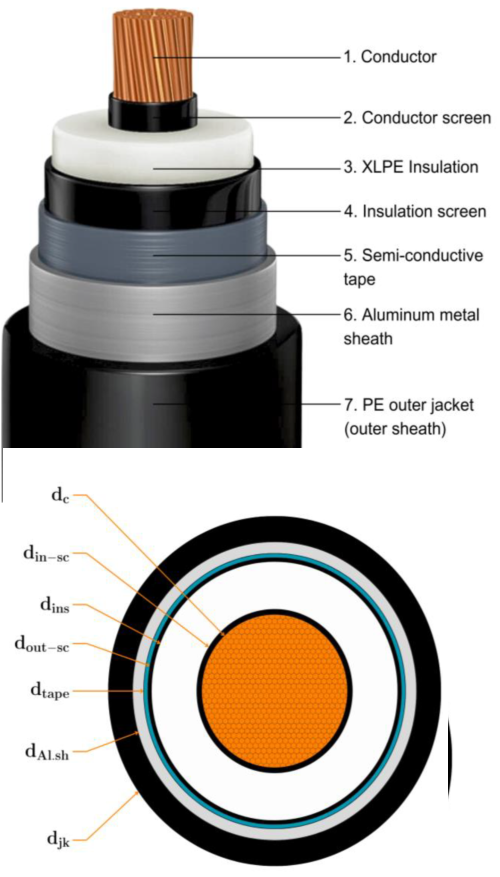
\includegraphics[height=0.27\textheight,keepaspectratio]{kim2025_cable_xsection}
\caption[Estructura multicapa de un cable XLPE]{Estructura multicapa de un cable XLPE usado como referencia del objeto de estudio. Fuente: \textcite[fig.~2]{kim2025}.}
\label{fig:cable-multicapa}
\end{figure}

La Figura~\ref{fig:zanja-cable}, basada en \textcite[fig.~1]{enescu2021}, muestra la segunda escala del objeto de estudio: la instalación enterrada. Allí el cable queda acoplado al material de relleno de la zanja, al \textit{bedding} cuando existe y al suelo nativo. Por ello, la conductividad térmica espacialmente variable $\kx$ no pertenece únicamente al cable, sino al sistema cable--instalación--entorno térmico, y debe representar la posición relativa de materiales con conductividades distintas.

\begin{figure}[htbp]
\centering
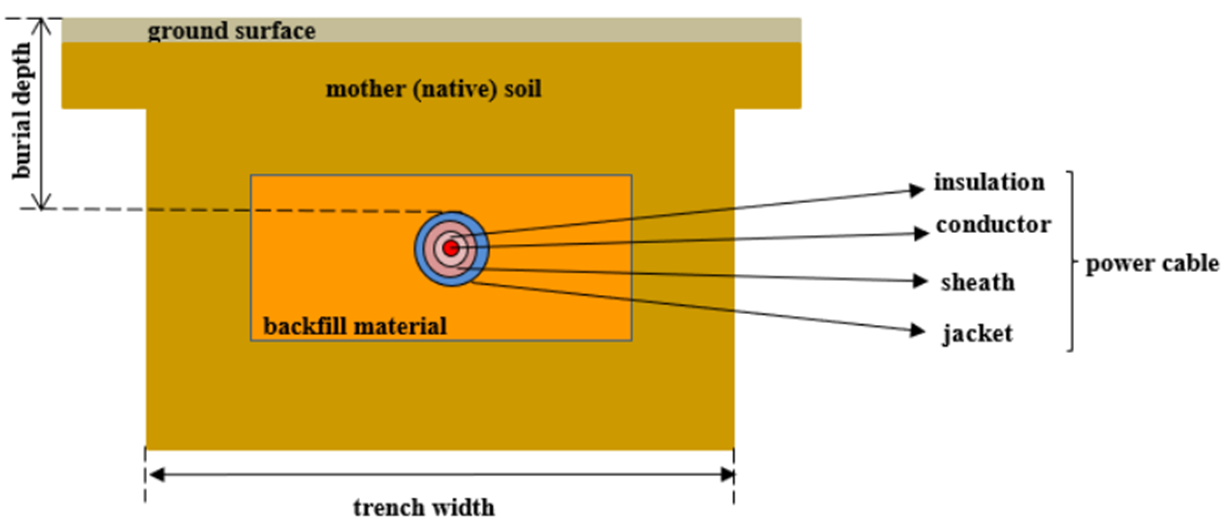
\includegraphics[width=0.97\textwidth,height=6.8cm,keepaspectratio]{enescu_trench_xsection}
\caption[Zanja y entorno térmico del cable enterrado]{Zanja y entorno térmico del cable enterrado: relleno, suelo nativo, profundidad de instalación y capas principales del cable. Fuente: \textcite[fig.~1]{enescu2021}.}
\label{fig:zanja-cable}
\end{figure}

\subsection{CONDUCTIVIDAD, RESISTIVIDAD Y HETEROGENEIDAD}
\label{subsec:conductividad-heterogeneidad}

La conductividad térmica expresa la facilidad para transferir calor y la resistividad es su inversa. En suelos, ambas dependen de composición, densidad y contenido de agua; el aumento de resistividad por secado observado por \textcite[1,7]{khumalo2025} muestra que puede formarse una zona local que actúa como barrera. El valor usado para diseño debe representar el estado de instalación y seguir procedimientos normalizados cuando proviene de ensayos o fuentes técnicas \parencite[secciones 4--6]{ieee442}.

Una propiedad promedio conserva cierta cantidad global, pero no necesariamente conserva la temperatura máxima ni la ubicación del punto caliente. Dos mapas con el mismo promedio pueden producir rutas de flujo distintas si una región aislante se ubica junto al cable o lejos de él. Esta es la razón física para estudiar $C_k$, $f_h$ y $d_h$ como dimensiones separadas.

Las interfaces también son parte del problema teórico. Cuando dos materiales están en contacto, el modelo debe conservar temperatura y flujo normal, salvo que se declare una resistencia de contacto. Esta condición, formulada en la Fórmula~\ref{for:interfaz}, evita que el cambio de material produzca saltos no físicos en el campo térmico \parencites{carslaw1959conduction,kakac2018heatConduction}{patankar1980numerical}[3]{xing2023}.

La Tabla~\ref{tab:base-teorica-uso} resume cómo estas bases se usan en otras partes del documento. Por tanto, el marco teórico cumple una función de enlace: explica la teoría y muestra cómo esa teoría se convierte en variables, fórmulas, métricas y anexos.

\begin{table}[htbp]
\centering
\caption{Relación entre base teórica y uso metodológico. Fuente: Elaboración propia.}
\label{tab:base-teorica-uso}
\begingroup
\footnotesize
\setlength{\tabcolsep}{3pt}
\renewcommand{\arraystretch}{1.25}
\begin{tabularx}{\textwidth}{L{3.2cm}Y Y}
\toprule
\textbf{Base teórica} & \textbf{Relación física} & \textbf{Uso en el estudio} \\
\midrule
Conductividad espacial $\kx$ & Controla el flujo de calor local según la ley de Fourier. & Factor principal en la sección~\ref{sec:dimensiones-operativas} y en el \ref{anx:diseno-factorial}. \\
Campo $T(x,y)$ & Solución de la ecuación de conducción para una geometría, fuentes y contornos dados. & Salida primaria del artefacto y base para las métricas de la sección~\ref{sec:metodologia}. \\
Temperatura máxima $\Tmax$ & Restricción térmica que resume la condición crítica del conductor. & Variable dependiente y criterio de error en la Fórmula~\ref{for:metricas-evaluacion}. \\
Ampacidad $\Imax$ & Corriente máxima compatible con el límite térmico adoptado. & Resultado operativo calculado con la condición de la Fórmula~\ref{for:ampacidad}. \\
Interfaces térmicas & Conservan temperatura y flujo entre materiales. & Requisito físico del artefacto y parte de la verificación de la sección~\ref{subsec:verificacion-dsr}. \\
\bottomrule
\end{tabularx}
\endgroup
\end{table}

\subsection{MÉTODOS DE CÁLCULO TÉRMICO}
\label{subsec:metodos-calculo-termico}

Los circuitos térmicos son rápidos e interpretables, pero requieren equivalencias geométricas, por lo que las revisiones de cables los distinguen de los métodos de solución de campo térmico \parencite[4--6]{enescu2021}. Los métodos numéricos de campo resuelven la PDE sobre una malla, una grilla o una partición del dominio. FEM aproxima la solución por elementos; FDM reemplaza derivadas por diferencias en una grilla; FVM integra balances sobre volúmenes de control y conserva flujos locales \parencites{patankar1980numerical}[3--4,93--99]{cigre2025}.

Estos métodos son útiles porque representan geometría, materiales, fuentes y contornos con mayor detalle que una equivalencia térmica global. Sin embargo, su credibilidad depende de propiedades, condiciones de borde, discretización, convergencia y verificación. Las PINN aproximan la solución con una red y diferenciación automática, pero trasladan parte de la dificultad a muestreo, ponderación de pérdidas y optimización \parencites[3--4,93--99]{cigre2025}[1--2,14--17]{lawal2022}.

Los métodos se tratarán como complementarios. Las normas IEC aportarán la referencia normativa, los casos FEM aportarán la referencia numérica del campo térmico y la PINN será el artefacto investigado. Por tanto, una discrepancia no se interpretará automáticamente como error de IEC o superioridad de PINN. Primero se revisarán supuestos, dominio y evidencia.

La Tabla~\ref{tab:metodos-calculo-termico} organiza esa complementariedad. Esta síntesis es importante porque la metodología no elige un método por preferencia, sino por función: norma para línea base, métodos de campo para referencia, casos analíticos para verificación y PINN como artefacto evaluado.

\begin{table}[htbp]
\centering
\caption{Función de los métodos térmicos dentro del estudio. Fuente: Elaboración propia a partir de \textcite{iec60287}, \textcite{iec60853}, \textcite[4--6]{enescu2021}, \textcite[3--4,93--99]{cigre2025}, \textcite{patankar1980numerical} y \textcite{raissi2019}.}
\label{tab:metodos-calculo-termico}
\begingroup
\footnotesize
\setlength{\tabcolsep}{3pt}
\renewcommand{\arraystretch}{1.25}
\begin{tabularx}{\textwidth}{L{3.1cm}Y Y}
\toprule
\textbf{Método o referencia} & \textbf{Aporte principal} & \textbf{Límite que justifica la evaluación} \\
\midrule
IEC y circuitos térmicos & Dan una base normativa e interpretable para corriente admisible. & Requieren equivalencias térmicas y pueden ocultar heterogeneidades locales. \\
Soluciones analíticas o manufacturadas & Permiten verificar el código frente a respuestas conocidas. & Cubren geometrías y condiciones idealizadas. \\
FEM & Representa geometría, materiales y contornos con detalle espacial. & Exige malla, convergencia y repetición del modelo para cada escenario. \\
FDM & Aproxima las derivadas de la PDE mediante diferencias en una grilla. & Es directo en dominios regulares, pero pierde flexibilidad ante geometrías e interfaces complejas. \\
FVM & Integra balances de energía sobre volúmenes de control. & Conserva flujos locales, pero requiere tratamiento cuidadoso de interfaces y contornos. \\
PINN & Integra PDE, contornos, interfaces y datos de referencia en una pérdida común. & Requiere controlar entrenamiento, pesos de pérdida, puntos de colocación y robustez. \\
\bottomrule
\end{tabularx}
\endgroup
\end{table}

\section{TÉCNICAS APLICADAS}
\label{sec:tecnicas-aplicadas}

\subsection{REDES NEURONALES INFORMADAS POR LA FÍSICA}
\label{subsec:pinn}

Una PINN, según la formulación de \textcite[686--690]{raissi2019}, representa una variable física mediante una red neuronal y usa diferenciación automática para calcular las derivadas que aparecen en la PDE. Los puntos de colocación permiten evaluar el residuo sin requerir una etiqueta de temperatura en cada punto. Si existen observaciones, pueden añadirse como otro término y convertir el problema en una combinación física--datos.

En términos de arquitectura, una PINN puede usar una red neuronal directa con entradas, capas ocultas, funciones de activación y una salida física. La diferencia central no está solo en la arquitectura, sino en el entrenamiento, porque la pérdida incorpora la PDE, los contornos y, cuando existen, datos de referencia \parencites[686--690]{raissi2019}[1--2,14--17]{lawal2022}.

Para el problema térmico, la red no aprende solo una relación empírica entre entradas y salidas. Aprende una aproximación $T_\theta$ que debe reducir el incumplimiento local de la ecuación de conducción, de modo que el residuo físico se convierte en evidencia de consistencia del modelo \parencites[686--690]{raissi2019}[1--2,14--17]{lawal2022}. La Fórmula~\ref{for:residuo-pinn-calor} se obtiene al evaluar la ecuación de calor con $T_\theta$ y reordenar sus términos como residuo.

\begin{formula}[htbp]
\centering
\begin{equation}
\label{for:residuo-pinn-calor}
r_f(x,y,t;\theta)=
\rho c_p\,\frac{\partial T_\theta}{\partial t}
-\nabla\!\cdot\!\left(k(x,y)\nabla T_\theta\right)
-q(x,y,t).
\end{equation}
\caption{Residuo físico de una PINN para conducción de calor.}
\end{formula}

La Fórmula~\ref{for:residuo-pinn-calor} debe interpretarse junto con contornos, interfaces y datos de referencia, cuando existan. Por ello, la metodología usa una función de pérdida compuesta, presentada en la Fórmula~\ref{for:loss}, y no una única métrica de ajuste. En esa pérdida, $\mathcal{L}_{\mathrm{PDE}}$ se calcula con el residuo en puntos de colocación, mientras que los otros términos conectan la solución con contornos, interfaces, datos y conservación de energía. Esta distinción es importante porque el estudio evaluará dominios multimateriales, donde la representación de interfaces y el balance entre términos de pérdida pueden condicionar el entrenamiento \parencites[16]{pan2025}[2--6]{ren2025}.

La Figura~\ref{fig:esquema-pinn-calor} resume ese mecanismo para el problema térmico. Primero, la red recibe coordenadas espaciales y, cuando corresponde, tiempo; luego, produce una aproximación del campo $T_\theta$. Después, la diferenciación automática calcula gradientes y derivadas temporales \parencite[686--690]{raissi2019}. Finalmente, la función de pérdida penaliza el incumplimiento de la ecuación de calor, contornos, interfaces, condición inicial y datos disponibles, de modo que el esquema sintetiza \textcite[686--690]{raissi2019}, \textcite[1--2,14--17]{lawal2022} y \textcite[1,3,16]{pan2025}.

\begin{figure}[htbp]
\centering
\begin{tikzpicture}[
  font=\footnotesize,
  node distance=0.50cm and 0.36cm,
  stage/.style={draw, rounded corners=3pt, align=center, text width=2.30cm,
                minimum height=1.05cm, fill=white, line width=0.45pt},
  model/.style={stage, fill=lightgray},
  residual/.style={stage, fill=lightblue, text width=2.86cm,
                   minimum height=1.55cm},
  total/.style={stage, fill=lightgray, text width=2.62cm,
                minimum height=1.15cm},
  output/.style={stage, text width=2.62cm, minimum height=1.05cm},
  group/.style={draw, dashed, rounded corners=4pt, inner sep=4pt,
                line width=0.4pt},
  arr/.style={-{Stealth[length=2.4mm]}, line width=0.45pt},
  feed/.style={-{Stealth[length=2.4mm]}, line width=0.45pt, dashed,
               rounded corners=2pt}
]
\node[stage] (input) {Entradas\\$(x,y,t)$; $k,\rho,c_p,q$\\contornos/datos};
\node[model, right=of input] (nn) {Red PINN\\capas ocultas\\activación\\$T_\theta(x,y,t)$};
\node[model, right=of nn] (auto) {Diferenciación\\automática\\$T_t,\nabla T,\nabla\!\cdot(k\nabla T)$};
\node[residual, right=of auto] (terms) {Pérdidas evaluadas\\[0.15em]
$r_f=\rho c_pT_t-\nabla\!\cdot(k\nabla T)-q$\\
$r_b,r_i$; $r_0,r_d$};
\node[total, right=of terms] (loss) {Pérdida total\\$\mathcal{L}=\sum_j\lambda_j\mathcal{L}_j$};
\node[output, below=0.62cm of auto] (out) {Salida evaluada\\campo de temperatura\\$T(x,y,t)$\\$\Tmax$, hotspot, $\Imax$};
\node[stage, below=0.62cm of loss] (opt) {Optimizador\\actualiza $\theta$};
\node[group, fit=(terms)(loss), label={[font=\scriptsize]above:Evaluación física y de datos}] (lossbox) {};
\coordinate (fbrail) at ($(out.south)+(0,-0.30cm)$);

\draw[arr] (input) -- (nn);
\draw[arr] (nn) -- (auto);
\draw[arr] (auto) -- (terms);
\draw[arr] (terms) -- (loss);
\draw[arr] (loss) -- (opt);
\draw[feed] (opt.south) |- (fbrail) -| (nn.south);
\draw[arr] (auto.south) -- (out.north);
\end{tikzpicture}
\caption[Esquema de funcionamiento de una PINN aplicada a conducción de calor]{Esquema de funcionamiento de una PINN aplicada a conducción de calor. Fuente: Elaboración propia a partir de \textcite{raissi2019}, \textcite{lawal2022} y \textcite{pan2025}.}
\label{fig:esquema-pinn-calor}
\end{figure}

Su utilidad para el estudio tiene tres razones: primero, ofrece una representación continua del campo; segundo, integra $\kx$; tercero, puede extenderse a identificación inversa. Sin embargo, sus riesgos también son claros, entre ellos el mal balance de pérdidas, las discontinuidades, los mínimos de optimización y el costo de entrenamiento \parencites[2--6]{ren2025}[16]{pan2025}.

Las técnicas de descomposición de dominio de \textcite[1--2]{shukla2021} aportan una ruta posible para tratar discontinuidades. Sin embargo, se incorporarán solo si el diseño básico demuestra que las necesita.

\subsection{CIENCIA DEL DISEÑO Y NATURALEZA DE LA CONTRIBUCIÓN}
\label{subsec:dsr-contribucion}

La metodología DSR busca conocimiento prescriptivo mediante artefactos útiles y evaluados. En este plan, el objeto físico es el sistema cable--instalación--entorno térmico bajo heterogeneidad.

El artefacto situado será el prototipo PINN usado para estudiar ese sistema. Además, la contribución abstracta incluirá requisitos, arquitectura, protocolo de evaluación y principios de diseño.

Estas categorías son coherentes con la tipología de \textcite[343--349]{gregor2013}. Por tanto, la investigación se posiciona como una mejora de métodos PINN aplicados a esta clase de problema.

Los principios iniciales son: conservar explícitamente la física; representar interfaces sin promediar de forma inadvertida; separar verificación de validación; mantener incertidumbre numérica por debajo del efecto analizado; y preservar trazabilidad de cada ejecución. Estos principios son proposiciones de diseño sujetas a evaluación y refinamiento, no conclusiones anticipadas.

En síntesis, el marco teórico reduce el problema a una cadena física y metodológica: $\kx$ modifica el flujo térmico, el flujo determina $T(x,y)$, $\Tmax$ limita la corriente admisible y la evaluación DSR exige verificar el artefacto antes de extraer principios de diseño. Esta cadena sostiene la metodología de la sección~\ref{sec:metodologia} y la organización del \ref{anx:operacionalizacion-variables} y del \ref{anx:diseno-factorial}.

\section{DEFINICIÓN DE TÉRMINOS}
\label{sec:definicion-terminos}

Esta sección precisa los términos que se usarán con sentido técnico u operacional en el estudio. Se incluyen aquellos que intervienen directamente en el problema, objetivos, hipótesis, dimensiones operativas, métricas o alcance del artefacto. Las definiciones tomadas de normas, literatura técnica o metodología DSR se citan; las definiciones operacionales se formulan para esta investigación y se apoyan en las fuentes que sustentan su uso.

\begingroup
\newcounter{terminodefinicion}
\renewcommand*\descriptionlabel[1]{\refstepcounter{terminodefinicion}\normalfont\bfseries\thesection.\theterminodefinicion. #1}
\begin{description}[style=nextline,itemsep=0.65\baselineskip,parsep=0pt,topsep=0.25\baselineskip]
  \item[Ampacidad.] Corriente máxima que puede transportar un cable sin superar el límite térmico adoptado para sus materiales y condiciones de instalación. Se denotará como $\Imax$ y se obtendrá al buscar la corriente que hace que $\Tmax$ alcance $T_{\mathrm{lim}}$ \parencites[752--760]{neher1957}{anders2005}[cláusulas 4--5]{iec60287}[3--6]{enescu2021}.

  \item[Ampacidad dinámica o DTR.] Estimación de la capacidad de corriente considerando la evolución temporal de carga, temperatura ambiente, suelo y estado térmico previo del cable. Se distingue de la ampacidad en régimen permanente porque aprovecha la inercia térmica del sistema y requiere supuestos transitorios explícitos \parencites[cláusulas 2--4]{iec60853}[3--6]{enescu2021}[14843--14845]{fariz2026}.

  \item[Artefacto.] Producto diseñado para resolver un problema relevante y generar conocimiento evaluable. Comprende la especificación, el prototipo PINN, los escenarios de prueba, las métricas y los principios de diseño derivados; se distingue del objeto de estudio físico, que es el sistema cable--instalación--entorno térmico \parencites[55--56]{peffers2007}[342--350]{gregor2013}.

  \item[Backfill.] Material de relleno colocado en la zanja alrededor del cable o sobre la zona de asiento. Puede tener propiedades térmicas distintas a las del suelo nativo y modificar la evacuación de calor del sistema cable--instalación--entorno térmico \parencites{anders2005}[1--3]{atoccsa2024}[1,10,16]{kim2025}[secciones 4--6]{ieee442}.

  \item[Bedding.] Material de asiento inmediato del cable dentro de la zanja. En el contexto del estudio se considera una región cercana al cable cuya conductividad, extensión y posición pueden afectar la temperatura máxima y el punto caliente \parencites[1--4]{oclon2015}[1,10,16]{kim2025}[secciones 4--6]{ieee442}.

  \item[Cable eléctrico enterrado.] Sistema multicapa instalado bajo tierra para transportar energía eléctrica. Su respuesta térmica depende de pérdidas internas, capas del cable, profundidad, configuración, relleno, suelo nativo y condiciones de frontera \parencites[752--760]{neher1957}{anders2005}[3--5]{enescu2020}[fig.~2]{kim2025}.

  \item[Caso de referencia o \textit{benchmark}.] Configuración con solución analítica, solución manufacturada, FEM convergente o resultado publicado que se usa para comparar y verificar el artefacto. Su función es aportar una base trazable para evaluar error, balance energético y consistencia física \parencites{cigre2022}[93--99]{cigre2025}.

  \item[Sistema cable--instalación--entorno térmico.] Objeto de estudio. Comprende el cable multicapa, su disposición de instalación, el \textit{bedding}, el \textit{backfill}, el suelo nativo, las condiciones de frontera y las fuentes de calor que determinan el campo de temperatura y la ampacidad \parencites[752--760]{neher1957}{anders2005}[3--5]{enescu2020}[4--6]{enescu2021}[1,10,16]{kim2025}.

  \item[Campo de temperatura.] Distribución espacial y, cuando corresponda, temporal de temperatura, representada como $T(x,y)$ o $T(x,y,t)$. Es la salida primaria del modelo y permite derivar $\Tmax$, punto caliente e $\Imax$ \parencites{carslaw1959conduction,kakac2018heatConduction,hahn2012heatConduction}[1,3,16]{pan2025}.

  \item[Ciencia del diseño o DSR.] Paradigma de investigación que diseña, demuestra y evalúa artefactos para resolver problemas prácticos y producir conocimiento prescriptivo. Estructura las fases de especificación, desarrollo, demostración, evaluación y comunicación \parencites[54--56]{peffers2007}[342--351]{gregor2013}[198--203]{delport2024}.

  \item[Condición de contorno.] Restricción impuesta en el borde del dominio de cálculo, por ejemplo temperatura prescrita, flujo de calor o intercambio convectivo equivalente. Su definición afecta la solución térmica y debe permanecer controlada en comparaciones pareadas \parencites{carslaw1959conduction,kakac2018heatConduction,hahn2012heatConduction}[3--5]{enescu2020}[3--4,93--99]{cigre2025}.

  \item[Conductividad térmica.] Propiedad $k$ que expresa la facilidad con la que un material conduce calor. En el modelo se usará como conductividad térmica espacialmente variable $\kx$ para representar cable, relleno, asiento y suelo con propiedades distintas \parencites{carslaw1959conduction,kakac2018heatConduction}{farouki1981thermal,devries1966thermal}[1,7]{khumalo2025}[secciones 4--6]{ieee442}.

  \item[Contraste de conductividad.] Relación o diferencia relativa entre conductividades de regiones del dominio. Se expresa mediante $C_k$ y se usa para ordenar escenarios de heterogeneidad baja, media o alta \parencites{farouki1981thermal,devries1966thermal}[1,6--9]{khumalo2025}[1,10,16]{kim2025}.

  \item[Ecuación de conducción de calor.] Ecuación de conservación de energía que relaciona capacidad térmica, conductividad, gradientes de temperatura y fuentes de calor. En régimen estacionario, la derivada temporal se anula; en régimen transitorio, se conserva el término de acumulación térmica \parencites{carslaw1959conduction,kakac2018heatConduction,hahn2012heatConduction}[1,3]{xing2023}[1,3,16]{pan2025}.

  \item[Ecuación diferencial en derivadas parciales o PDE.] Ecuación que involucra derivadas de una función respecto de varias variables independientes. La PDE principal del modelo es la ecuación de conducción de calor y su residuo se incorpora a la pérdida de la PINN \parencites[686--690]{raissi2019}[1--2]{lawal2022}.

  \item[Extensión de heterogeneidad.] Tamaño o fracción del dominio afectado por una región con conductividad distinta a la base. Se representa mediante $f_h$ y se evalúa junto con contraste y proximidad \parencites[4--6]{enescu2021}[1,6--9]{khumalo2025}[1,10,16]{kim2025}.

  \item[FEM.] Método de elementos finitos. Discretiza el dominio en elementos para aproximar el campo de temperatura en geometrías y materiales complejos. Funcionará como referencia numérica convergente del campo térmico, no como artefacto principal \parencites[4--6]{enescu2021}{patankar1980numerical}[3--4,93--99]{cigre2025}.

  \item[FDM.] Método de diferencias finitas. Aproxima las derivadas de una PDE mediante diferencias entre nodos de una grilla. Es útil para dominios regulares, aunque puede volverse menos flexible cuando existen geometrías o interfaces complejas \parencites{patankar1980numerical}[3--4,93--99]{cigre2025}.

  \item[FVM.] Método de volúmenes finitos. Integra la ecuación de balance sobre volúmenes de control y calcula flujos entre celdas. Es útil cuando se requiere conservación local, pero exige definir con cuidado interfaces, contornos y propiedades de celda \parencite{patankar1980numerical}.

  \item[Función de pérdida.] Función objetivo minimizada durante el entrenamiento de la PINN. Combina residuos de PDE, contornos, interfaces, condición inicial y, si existen, datos de referencia, ponderados por coeficientes $\lambda_j$ \parencites[686--690]{raissi2019}[16]{pan2025}[1--2,17]{lawal2022}.

\item[Heterogeneidad térmica.] Variación espacial de propiedades térmicas dentro del dominio. El análisis se centra en la conductividad térmica espacialmente variable $\kx$ del sistema cable--instalación--entorno térmico y se caracteriza por contraste, patrón, extensión y proximidad al conductor \parencites{farouki1981thermal,devries1966thermal}[4--6]{enescu2021}[1,6--9]{khumalo2025}[1,10,16]{kim2025}.

  \item[Interfaz térmica.] Frontera interna entre materiales con propiedades térmicas distintas. Para el modelo se exigirá continuidad de temperatura y de flujo normal, salvo que el caso de referencia especifique una resistencia de contacto \parencites{carslaw1959conduction,kakac2018heatConduction,hahn2012heatConduction}{patankar1980numerical}[3]{xing2023}[3--4,93--99]{cigre2025}.

  \item[Material PAC.] Agregado de concreto premezclado usado como relleno con propiedades térmicas mejoradas. Se considera un ejemplo de \textit{backfill} de mayor conductividad que puede reducir la temperatura del conductor respecto de la arena natural \parencite[1,10,16]{kim2025}.

  \item[PINN.] Red neuronal informada por física. Aproxima una variable física mediante una red neuronal y penaliza el incumplimiento de la PDE y de condiciones auxiliares durante el entrenamiento \parencites[686--690]{raissi2019}[1--2,14--17]{lawal2022}[1,3,16]{pan2025}.

  \item[Polietileno reticulado o XLPE.] Material aislante usado en cables de potencia. Su límite térmico condiciona la temperatura admisible del conductor y, por tanto, el cálculo de ampacidad \parencites{iec60502_2_2014}[3--5]{enescu2020}[fig.~2]{kim2025}.

  \item[Proximidad de heterogeneidad.] Distancia entre una región heterogénea y el conductor o zona de mayor generación de calor. Se representa mediante $d_h$ y permite distinguir si una anomalía térmica está cerca, a distancia intermedia o lejos del cable \parencites[1,6--9]{khumalo2025}[1,10,16]{kim2025}[1--4]{oclon2015}.

  \item[Punto caliente.] Ubicación del dominio donde el campo de temperatura alcanza el máximo relevante para operación o diseño. Se registrará mediante sus coordenadas $(x_h,y_h)$ y se comparará entre escenarios homogéneos y heterogéneos \parencites[1,6--9]{khumalo2025}[1,10,16]{kim2025}.

  \item[Punto de colocación.] Punto del dominio o del contorno usado para evaluar la PDE, las condiciones de borde o las condiciones de interfaz durante el entrenamiento de una PINN. No requiere necesariamente una etiqueta de temperatura de referencia \parencites[686--690]{raissi2019}[1--2]{lawal2022}.

  \item[Representación homogénea equivalente.] Sustitución de un entorno heterogéneo por una propiedad térmica única o promedio. Se usará como referencia de comparación para cuantificar cuánto cambian $\Tmax$ e $\Imax$ al representar explícitamente la conductividad térmica espacialmente variable $\kx$ \parencites{farouki1981thermal,devries1966thermal}[4--6]{enescu2021}[3--4,41--42,93--99]{cigre2025}.

  \item[Residuo físico.] Incumplimiento local de la ecuación gobernante o de una condición auxiliar al evaluar la aproximación del campo de temperatura $T_\theta$. En la PINN, los residuos forman términos de la función de pérdida y sirven como indicadores de consistencia física \parencites[686--690]{raissi2019}[1--2,14--17]{lawal2022}.

  \item[Resistividad térmica.] Inversa de la conductividad térmica, usualmente expresada en \si{\kelvin\metre\per\watt}. En suelos y rellenos depende de composición, densidad y humedad, por lo que puede cambiar significativamente entre condición húmeda y seca \parencites{farouki1981thermal,devries1966thermal}[1,6--9]{khumalo2025}[secciones 4--6]{ieee442}.

  \item[Solución manufacturada.] Solución artificial definida de antemano para un problema de verificación numérica. A partir de ella se construyen fuentes o condiciones de contorno compatibles, de modo que el error del artefacto pueda evaluarse contra una respuesta conocida \parencites{cigre2022}[93--99]{cigre2025}.

  \item[Suelo nativo.] Material natural existente alrededor de la zanja antes de incorporar asiento o relleno. Sus propiedades térmicas dependen de composición, densidad y humedad, y constituyen una parte central del entorno térmico del cable enterrado \parencites{farouki1981thermal,devries1966thermal}[1,6--9]{khumalo2025}[secciones 4--6]{ieee442}.

  \item[Temperatura máxima del conductor.] Máximo valor de temperatura en la región del conductor, denotado $\Tmax$. Es la variable térmica principal para verificar el cumplimiento de $T_{\mathrm{lim}}$ y calcular $\Imax$ \parencites[752--760]{neher1957}{anders2005}[cláusulas 4--5]{iec60287}[3--6]{enescu2021}.

  \item[Validación.] Evaluación de si el modelo representa con suficiencia una instalación real o el caso de uso declarado mediante evidencia empírica independiente. No se realizará validación experimental de campo; el término se reserva para trabajos que incluyan instrumentación, medición de propiedades del suelo, registro de carga y temperatura, y seguimiento operativo de una instalación real \parencites{cigre2022}[93--99]{cigre2025}[350--351]{gregor2013}.

  \item[Verificación.] Evaluación de si la formulación matemática, el código y el procedimiento numérico resuelven correctamente el problema especificado. Incluye casos analíticos simples, soluciones manufacturadas, referencias FEM convergentes, casos publicados con datos comparables, balance energético, residuos, contornos e interfaces \parencites{cigre2022}[3--4,93--99]{cigre2025}[350--351]{gregor2013}.

  \item[Zona seca.] Región de suelo o relleno con bajo contenido de humedad y mayor resistividad térmica que el material en condición húmeda. Puede aparecer por condiciones ambientales o calentamiento y reducir la disipación de calor del cable \parencites[4--6]{enescu2021}[1,6--9]{khumalo2025}[14851--14852]{fariz2026}.
\end{description}
\endgroup

% ===========================================================================
\begin{singlespace}
\tesisbodyfont
\printbibliography[heading=subbibnumbered,title={REFERENCIAS}]
\end{singlespace}

% ===========================================================================
\begin{singlespace}
\tesisbodyfont
\renewcommand{\thesection}{ANEXO \thechapter.\arabic{section}}
\titleformat{\section}
  {\normalfont\bfseries\fontsize{11}{13.2}\selectfont}
  {\thesection.}{0.75em}{\MakeUppercase}
\titlespacing*{\section}{0pt}{1.0\baselineskip}{0.25\baselineskip}
\begin{landscape}
\chapter{ANEXOS}
\thispagestyle{empty}

Los anexos reúnen organizadores, matrices y registros que sostienen la trazabilidad del plan. Por tanto, no funcionan como material aislado, sino como respaldo de la relación entre problema, método, evidencia y evaluación.

\section{MATRIZ DE CONSISTENCIA}
\thispagestyle{empty}
\scriptsize
La matriz articula los problemas de investigación con los objetivos, productos verificables, insumos, resultados, hipótesis y evidencia de evaluación del artefacto. Los problemas se formulan como enunciados narrativos, de modo que cada fila exprese una carencia verificable que será atendida por el diseño, implementación, evaluación y comunicación del artefacto PINN 2D.

La Tabla~\ref{tab:matriz-consistencia-a} presenta la primera parte de la matriz y verifica la correspondencia entre cada fase DSR, el problema que atiende, el objetivo asociado y el producto que permitirá comprobar su avance.

% ---------------------------------------------------------------------------
% Tabla 1: Desde fase/actividad hasta producto verificable
% ---------------------------------------------------------------------------
\setlength{\tabcolsep}{3pt}
\renewcommand{\arraystretch}{1.18}

\begin{longtable}{%
L{3.8cm}
L{6.2cm}
L{5.3cm}
L{5.0cm}}
\caption{Matriz de consistencia del plan de tesis: problema, objetivo y producto verificable.}
\label{tab:matriz-consistencia-a}\\
\toprule
\textbf{Fase DSR / actividad} &
\textbf{Problema} &
\textbf{Objetivo} &
\textbf{Producto verificable} \\
\midrule
\endfirsthead

\toprule
\textbf{Fase DSR / actividad} &
\textbf{Problema} &
\textbf{Objetivo} &
\textbf{Producto verificable} \\
\midrule
\endhead

\midrule
\multicolumn{4}{r}{\small Continúa en la siguiente página.}\\
\midrule
\endfoot

\bottomrule
\endlastfoot

\textbf{F0. Definición del objeto de estudio, caso de uso y alcance del artefacto} &
\textbf{PG. Estimación y decisión:} pese a la disponibilidad de técnicas para estimar temperatura y ampacidad en cables eléctricos subterráneos, los casos con entorno térmicamente heterogéneo mantienen una limitación práctica: las representaciones homogéneas equivalentes son rápidas, pero no describen explícitamente la conductividad térmica espacialmente variable $\kx$, mientras que los modelos FEM pueden representar esa heterogeneidad, pero exigen construir, mallar, verificar y repetir modelos para cada escenario a un alto costo computacional. Por ello, resulta difícil cuantificar de forma reproducible y trazable cómo la heterogeneidad del suelo y el entorno del cable enterrado modifica el campo de temperatura $T(x,y)$, la temperatura máxima $\Tmax$ y la ampacidad $\Imax$ frente a una representación homogénea equivalente. &
\textbf{OG.} Diseñar y evaluar un artefacto PINN 2D para estudiar, de forma reproducible y trazable, el sistema cable--instalación--entorno térmico en cables eléctricos subterráneos, estimar el campo de temperatura $T(x,y)$, determinar $\Tmax$ e $\Imax$ y cuantificar el efecto de la heterogeneidad térmica espacial del entorno. &
Protocolo general del artefacto; dominio de validez; criterios de aceptación; repositorio de escenarios y resultados. \\

\midrule
\textbf{F1. Especificación física, datos y requisitos} &
\textbf{PE1. Especificación:} no está formalizado qué información física, funcional y de calidad debe ingresar al artefacto para representar cable multicapa, interfaces, fuentes térmicas, condiciones de contorno y conductividad térmica espacialmente variable $\kx$ en escenarios heterogéneos de cables enterrados. &
\textbf{OE1.} Especificar las entradas físicas, requisitos funcionales y criterios de calidad del artefacto para representar el sistema cable--instalación--entorno térmico, incluyendo dominios multicapa, fuentes térmicas, condiciones de contorno, interfaces y conductividad térmica espacialmente variable $\kx$. &
Documento de requisitos; catálogo de materiales y geometrías; ficha de supuestos; matriz de trazabilidad requisito--prueba. \\

\midrule
\textbf{F2. Preparación de datos sintéticos, geometría y referencias} &
\textbf{PE2. Referencia y verificación:} no se dispone de un paquete reproducible de referencias analíticas, manufacturadas, FEM y casos publicados que sirva como insumo de verificación antes de usar el artefacto para estimar ampacidad. &
\textbf{OE2.} Construir y verificar el artefacto usando como insumos soluciones analíticas o manufacturadas, benchmarks FEM con convergencia y casos publicados. &
Base de benchmarks; casos manufacturados; mallas o soluciones FEM convergentes; informe de verificación. \\

\midrule
\textbf{F3. Experimentación numérica y análisis de sensibilidad} &
\textbf{PE3. Sensibilidad térmica:} no existe una evaluación trazable que, a partir de escenarios controlados de contraste, patrón, extensión y proximidad de heterogeneidades del suelo y los rellenos, entregue como resultado el cambio en $\Tmax$, el campo de temperatura $T(x,y)$ y la localización del punto caliente. &
\textbf{OE3.} Evaluar escenarios controlados de contraste, patrón, extensión y proximidad de heterogeneidades del suelo y los rellenos para obtener cambios en $\Tmax$, el campo de temperatura $T(x,y)$ y la localización del punto caliente. &
Plan de experimentación numérica DSR; mapas de conductividad térmica espacialmente variable $\kx$; resultados de sensibilidad; curvas y mapas de temperatura; informe de efectos físicos y límites del artefacto. \\

\midrule
\textbf{F4. Evaluación de ampacidad y comparación de escenarios} &
\textbf{PE4. Decisión operativa:} no están identificadas las condiciones de entrada bajo las cuales una representación homogénea equivalente produce la mayor discrepancia de ampacidad frente a una representación 2D heterogénea verificada. &
\textbf{OE4.} Comparar la ampacidad obtenida con representación 2D heterogénea frente a escenarios homogéneos equivalentes e identificar las condiciones de entrada que generan mayor discrepancia. &
Rutina de búsqueda de $\Imax$; tabla de \textit{derating}/\textit{uprating}; ranking de escenarios críticos; comparación heterogéneo--homogéneo. \\

\midrule
\textbf{F5. Síntesis y reproducibilidad} &
\textbf{PE5. Transferencia y reproducibilidad:} no se ha sistematizado, a partir de la evidencia generada por el artefacto, un procedimiento reproducible ni principios transferibles para analizar esta clase de problemas 2D multimateriales sin rehacer manualmente todo el proceso de modelado numérico para cada escenario. &
\textbf{OE5.} Formular, a partir de los resultados del artefacto, principios de diseño y un procedimiento reproducible para aplicar y evaluar PINN en problemas térmicos multimateriales de cables enterrados. &
Repositorio depurado; bitácora de versiones; guía de reproducción; principios de diseño; informe final de evaluación DSR. \\

\end{longtable}

\vspace{0.6cm}

La Tabla~\ref{tab:matriz-consistencia-b} completa la matriz con factores independientes, niveles de configuración, resultados dependientes, hipótesis, evidencia y controles. Su función es mostrar cómo cada problema se vuelve observable dentro del ciclo DSR y cómo se evitará atribuir efectos a la conductividad térmica espacialmente variable $\kx$ cuando dependan de geometría, pérdidas, contornos o configuración numérica.

% ---------------------------------------------------------------------------
% Tabla 2: Factores, resultados, hipótesis, evidencia y controles
% ---------------------------------------------------------------------------
\setlength{\tabcolsep}{1pt}
\renewcommand{\arraystretch}{1.15}

\begin{longtable}{%
L{2.55cm}
L{3.20cm}
L{2.25cm}
L{3.10cm}
L{2.35cm}
L{4.00cm}
L{3.00cm}
L{3.10cm}}
\caption{Matriz de consistencia del plan de tesis: factores, resultados, hipótesis, evidencia y controles.}
\label{tab:matriz-consistencia-b}\\
\toprule
\textbf{Fase DSR / actividad} &
\textbf{Problema} &
\textbf{Factor o entrada independiente} &
\textbf{Nivel o configuración del factor} &
\textbf{Resultado dependiente esperado} &
\textbf{Hipótesis} &
\textbf{Evidencia o indicadores de evaluación} &
\textbf{Condiciones de control} \\
\midrule
\endfirsthead

\toprule
\textbf{Fase DSR / actividad} &
\textbf{Problema} &
\textbf{Factor o entrada independiente} &
\textbf{Nivel o configuración del factor} &
\textbf{Resultado dependiente esperado} &
\textbf{Hipótesis} &
\textbf{Evidencia o indicadores de evaluación} &
\textbf{Condiciones de control} \\
\midrule
\endhead

\midrule
\multicolumn{8}{r}{\small Continúa en la siguiente página.}\\
\midrule
\endfoot

\bottomrule
\endlastfoot

\textbf{F0. Definición del objeto de estudio, caso de uso y alcance del artefacto} &
\textbf{PG. Estimación y decisión.} &
Representación térmica del sistema de cable enterrado y de la conductividad térmica espacialmente variable $\kx$. &
Homogénea equivalente; estratificada; inclusión localizada; \textit{bedding}; \textit{backfill}; zona seca; combinaciones multimateriales. &
Campo de temperatura $T(x,y)$, $\Tmax$, $\Imax$, dominio de validez y protocolo general del artefacto. &
\textbf{HG.} La incorporación explícita de la conductividad térmica espacialmente variable $\kx$ en una PINN 2D permitirá reproducir referencias verificadas con error de ingeniería controlado, evidenciar diferencias sistemáticas de temperatura máxima y ampacidad frente a un entorno homogéneo equivalente cuando existan regiones de baja o alta conductividad próximas al cable, y reportar la trazabilidad y el costo computacional del proceso. &
$e_{\Tmax}$; NRMSE espacial; $\Delta\Tmax$; $\Delta I\pct$; desequilibrio energético; robustez entre semillas; tiempo de cómputo. &
Geometría del cable; profundidad; disposición; pérdidas; $T_{\mathrm{amb}}$; tamaño del dominio; condiciones de borde; límite térmico $T_{\mathrm{lim}}$; hardware y versión del código. \\

\midrule
\textbf{F1. Especificación física, datos y requisitos} &
\textbf{PE1. Especificación.} &
Entradas físicas, funcionales y de calidad requeridas para representar el sistema térmico estudiado. &
Sin especificación; especificación parcial; especificación completa y trazable. &
Requisitos verificables, matriz requisito--prueba y criterios de aceptación del artefacto. &
\textbf{HE1.} Una especificación que separe PDE, contornos, interfaces, fuentes y propiedades térmicas reducirá ambigüedades de implementación y permitirá definir pruebas verificables de consistencia física y funcional. &
Porcentaje de requisitos críticos cubiertos; número de pruebas asociadas por requisito; trazabilidad completa/incompleta; cumplimiento de unidades y supuestos. &
Normas y fuentes usadas; sistema de unidades; geometría base; materiales incluidos; alcance estacionario/transitorio; exclusiones declaradas. \\

\midrule
\textbf{F2. Preparación de datos sintéticos, geometría y referencias} &
\textbf{PE2. Referencia y verificación.} &
Tipo y calidad de la referencia usada para verificar el artefacto. &
Solución analítica; solución manufacturada; FEM convergente; caso publicado; escenario sin referencia. &
Errores de verificación, consistencia física y paquete reproducible de benchmarks. &
\textbf{HE2.} El artefacto alcanzará, dentro del dominio de verificación, error relativo de $\Tmax$ no mayor a 5\,\pct{}, NRMSE no mayor a 5\,\pct{} y desequilibrio energético no mayor a 2\,\pct{} frente a referencias convergentes. &
$e_{\Tmax}$; MAE; RMSE/NRMSE; error máximo; residuo PDE; error de contorno; error de interfaz; balance de energía; CV de $\Tmax$. &
Densidad de puntos de colocación; semilla; arquitectura; pesos de pérdida; tolerancia FEM; tamaño de malla; criterio de convergencia; dominio físico. \\

\midrule
\textbf{F3. Experimentación numérica y análisis de sensibilidad} &
\textbf{PE3. Sensibilidad térmica.} &
Conductividad térmica espacialmente variable $\kx$ como factor independiente principal. &
Contraste bajo/medio/alto $C_k$; proximidad cercana/media/lejana $d_h$; extensión pequeña/media/grande $f_h$; patrón estratificado/localizado/relleno/zona seca. &
Mapas térmicos y efectos sobre $\Tmax$, punto caliente y campo de temperatura $T(x,y)$. &
\textbf{HE3.} A igualdad de geometría, pérdidas y contornos, una región de baja $k$ más extensa y próxima al conductor aumentará $\Tmax$ y desplazará el punto caliente; una región de alta $k$ usada como relleno reducirá $\Tmax$. &
$\Delta\Tmax$; coordenadas del punto caliente $(x_h,y_h)$; $|\nabla T|_{\max}$; cambio de temperatura media; tamaño de efecto; intervalos por repetición. &
Corriente o pérdidas; profundidad; disposición; $T_{\mathrm{amb}}$; tamaño del dominio; condiciones de borde; arquitectura y entrenamiento congelados tras piloto. \\

\midrule
\textbf{F4. Evaluación de ampacidad y comparación de escenarios} &
\textbf{PE4. Decisión operativa.} &
Representación térmica del entorno usada para calcular ampacidad. &
Representación explícita de la conductividad térmica espacialmente variable $\kx$; homogénea equivalente por promedio; homogénea conservadora; homogénea optimista. &
Ampacidad $\Imax$, margen térmico y ranking de discrepancias. &
\textbf{HE4.} La aproximación homogénea tenderá a sobreestimar $\Imax$ cuando promedie una zona local de baja $k$ cercana al cable, y la discrepancia crecerá con el contraste y la extensión de esa zona. &
$\Imax$; $\Delta I\pct$; margen respecto de $T_{\mathrm{lim}}$; número de iteraciones de búsqueda; incertidumbre combinada modelo--referencia. &
Criterio de $T_{\mathrm{lim}}$; pérdidas dependientes de corriente; paso/tolerancia de bisección; geometría; condiciones de borde; referencia homogénea adoptada. \\

\midrule
\textbf{F5. Síntesis y reproducibilidad} &
\textbf{PE5. Transferencia y reproducibilidad.} &
Nivel de trazabilidad y empaquetamiento de la evidencia generada por el artefacto. &
Prototipo no reproducible; prototipo reproducible localmente; paquete documentado; paquete con pruebas automatizadas y trazabilidad completa. &
Procedimiento reproducible, principios de diseño y paquete documentado. &
\textbf{HE5.} Los principios y procedimientos extraídos del artefacto serán aplicables a una clase de problemas 2D multimaterial y no únicamente a una configuración individual, si preservan trazabilidad, pruebas, límites de validez y métricas de calidad. &
Reproducibilidad de casos aceptados; cobertura de pruebas; trazabilidad de datos/código/resultados; completitud documental; estabilidad de resultados; tiempo de reconstrucción. &
Sistema operativo; versión de bibliotecas; hardware; semillas; formato de datos; política de nombres; control de versiones; disponibilidad legal de fuentes y datos. \\

\end{longtable}
\end{landscape}

\clearpage
\tesisbodyfont

\begin{landscape}
\section{MATRIZ DE OPERACIONALIZACIÓN DE VARIABLES}
\label{anx:operacionalizacion-variables}
\thispagestyle{empty}

Este anexo traduce las dimensiones operativas del estudio a la nomenclatura metodológica de variables independientes, variables dependientes, controles e instrumentos de registro y evaluación. La intención no es forzar la investigación a un experimento estadístico clásico, sino dejar claro qué se modifica, qué se observa, qué se mantiene constante y con qué evidencia se sostendrá cada resultado.

\footnotesize
\setlength{\tabcolsep}{3pt}
\renewcommand{\arraystretch}{1.18}
\begin{longtable}{L{4.00cm}L{4.20cm}L{8.20cm}L{6.30cm}}
\caption{Matriz de operacionalización de variables.}
\label{tab:operacionalizacion-variables}\\
\toprule
\textbf{Elemento metodológico} &
\textbf{Variable, factor o resultado} &
\textbf{Operacionalización en el estudio} &
\textbf{Indicador, instrumento o registro} \\
\midrule
\endfirsthead

\toprule
\textbf{Elemento metodológico} &
\textbf{Variable, factor o resultado} &
\textbf{Operacionalización en el estudio} &
\textbf{Indicador, instrumento o registro} \\
\midrule
\endhead

\midrule
\multicolumn{4}{r}{\small Continúa en la siguiente página.}\\
\midrule
\endfoot

\bottomrule
\endlastfoot

Sistema estudiado & Sistema cable--instalación--entorno térmico & Instalación enterrada en la que el conductor genera calor y lo disipa hacia capas de cable, relleno, asiento y suelo. & Ficha del caso; geometría; materiales; carga; condiciones de borde. \\

Objeto de estudio & Comportamiento térmico y operativo ante heterogeneidad & Relación entre la representación espacial de $\kx$ y las respuestas $T(x,y)$, $\Tmax$ e $\Imax$. & Comparación entre escenario heterogéneo y escenario homogéneo equivalente. \\

Unidad de análisis & Sección transversal 2D del sistema & Caso computacional parametrizado por geometría, materiales, fuentes, contornos, referencia y versión del artefacto. & Identificador de caso; archivo de entrada; metadatos de ejecución; salida reproducible. \\

Variable independiente principal & Conductividad térmica espacialmente variable $\kx$ & Mapa de conductividad asignado al suelo, \textit{bedding}, \textit{backfill} o zona seca, según el patrón de heterogeneidad evaluado. & $k$ por material; contraste $C_k$; mapa $\kx$; fuente bibliográfica o supuesto declarado. \\

Factores independientes derivados & Contraste, patrón, extensión y proximidad & Niveles combinados para construir escenarios de sensibilidad y comparación factorial. & $C_k$; patrón $P$; fracción o tamaño $f_h$; distancia normalizada $d_h/D$. \\

Variable dependiente térmica & Campo de temperatura y temperatura máxima & Respuesta calculada por la PINN y comparada con referencia analítica, manufacturada, FEM o publicada cuando exista. & $T(x,y)$; $\Tmax$; $\Delta\Tmax$; punto caliente; MAE; RMSE; NRMSE. \\

Variable dependiente operativa & Ampacidad y margen térmico & Corriente máxima compatible con $T_{\mathrm{lim}}$ y diferencia frente a la representación homogénea equivalente. & $\Imax$; $\Delta I\pct$; \textit{derating}; \textit{uprating}; número de iteraciones de búsqueda. \\

Resultado de evaluación del artefacto & Exactitud, consistencia, utilidad y reproducibilidad & Calidad técnica del artefacto dentro del ciclo DSR, no solo valor numérico de una simulación aislada. & Residuo PDE; error de contorno e interfaz; balance energético; robustez entre semillas; tiempo de cómputo. \\

Variables controladas & Geometría, pérdidas, contornos y configuración numérica & Condiciones que se fijan dentro de cada comparación pareada para atribuir el cambio observado a $\kx$. & Diámetros; profundidad; separación; corriente o pérdidas; $T_{\mathrm{amb}}$; dominio; arquitectura; pesos de pérdida tras piloto. \\

Variables no controladas registradas & Incertidumbre documental y variabilidad numérica & Condiciones que no siempre pueden fijarse, pero que se reportan para interpretar la evidencia sin ocultar limitaciones. & Semilla; convergencia; tolerancia FEM; datos faltantes de publicaciones; rango de propiedades térmicas; hardware. \\

Instrumento de registro y evaluación & Artefacto PINN y protocolo de verificación & Conjunto formado por especificación, implementación, casos de referencia, scripts de evaluación, bitácora y repositorio. & Código versionado; archivos parametrizados; pruebas; tablas de resultados; figuras térmicas; bitácora DSR. \\

Característica de registro & Registro computacional del campo térmico y métricas escalares & Registro de matrices espaciales, máximos, diferencias porcentuales, residuos, tiempos y metadatos. & Matrices $T(x,y)$; mapas $\kx$; CSV de métricas; reporte de energía; salida gráfica. \\

Tamaño de muestra metodológico & Paquete de casos y escenarios & Conjunto de casos de verificación y escenarios factoriales definidos por pertinencia técnica y costo computacional. & Casos analíticos/manufacturados; benchmarks FEM; casos publicados; bloque factorial del \ref{anx:diseno-factorial}. \\

\end{longtable}
\end{landscape}

\tesisbodyfont

\clearpage
\begin{landscape}
\section{DISEÑO FACTORIAL}
\label{anx:diseno-factorial}
\thispagestyle{empty}

Este anexo precisa el diseño factorial que se usará para estudiar la heterogeneidad térmica. No corresponde a un análisis factorial exploratorio de variables latentes; se trata de un diseño factorial de escenarios numéricos. En otras palabras, se combinan niveles de factores físicos para observar cómo cambia la temperatura y la ampacidad cuando el entorno deja de ser homogéneo.

\scriptsize
\setlength{\tabcolsep}{3pt}
\renewcommand{\arraystretch}{1.18}
\begin{longtable}{L{2.65cm}L{1.35cm}L{5.1cm}L{5.1cm}L{5.2cm}}
\caption{Diseño Factorial.}
\label{tab:analisis-factorial}\\
\toprule
\textbf{Factor} &
\textbf{Código} &
\textbf{Niveles iniciales} &
\textbf{Sentido físico} &
\textbf{Resultado que permite observar} \\
\midrule
\endfirsthead

\toprule
\textbf{Factor} &
\textbf{Código} &
\textbf{Niveles iniciales} &
\textbf{Sentido físico} &
\textbf{Resultado que permite observar} \\
\midrule
\endhead

\midrule
\multicolumn{5}{r}{\small Continúa en la siguiente página.}\\
\midrule
\endfoot

\bottomrule
\endlastfoot

Patrón de heterogeneidad & $P$ & Estratificado; inclusión localizada de baja $k$; relleno de alta $k$; zona seca parcial. & Describe la forma espacial en que el entorno térmico deja de ser homogéneo. & Permite separar si el efecto proviene de una capa, una bolsa local, un material de mejora térmica o una zona seca. \\

Contraste térmico & $C_k$ & Bajo; medio; alto, definido como razón de conductividades respecto del entorno base. & Mide qué tan distinta es la región heterogénea frente al suelo o relleno de referencia. & Efecto principal sobre $\Tmax$, gradiente térmico y margen operativo. \\

Extensión de la región heterogénea & $f_h$ & Pequeña; media; grande, expresada como fracción del entorno local o tamaño normalizado. & Representa cuánto volumen alrededor del cable participa en la barrera o mejora térmica. & Cambio en $\Delta\Tmax$, tamaño del punto caliente y sensibilidad del campo $T(x,y)$. \\

Proximidad al conductor & $d_h$ & Cercana; media; lejana, normalizada por el diámetro exterior del cable o distancia característica $D$. & Ubica la heterogeneidad respecto de la zona donde el flujo térmico es más intenso. & Interacción entre posición y contraste; desplazamiento del punto caliente. \\

Representación de comparación & $R$ & Heterogénea explícita; homogénea equivalente; homogénea conservadora; homogénea optimista. & Permite contrastar el artefacto con simplificaciones usadas en cálculo de ampacidad. & Diferencia de ampacidad $\Delta I\pct$ y ranking de escenarios críticos. \\

Semilla o repetición numérica & $S$ & Repeticiones seleccionadas en piloto y casos extremos. & No es factor físico; mide robustez de entrenamiento del artefacto PINN. & Variabilidad de $\Tmax$, error, convergencia y tiempo de cómputo. \\

\end{longtable}

\tesisbodyfont

El bloque factorial principal combinará $C_k$, $f_h$ y $d_h$ dentro de cada patrón $P$. Con tres niveles por factor se obtiene un bloque base de $3^3=27$ escenarios por patrón.

Si se evalúan los cuatro patrones iniciales, el bloque completo tendrá 108 escenarios heterogéneos. Además, cada escenario se comparará con su referencia homogénea correspondiente.

Este número se entiende como marco de planificación. Por tanto, si el piloto muestra un costo excesivo, se conservarán completos los patrones más críticos y se justificará cualquier fracción usada.

La lectura de resultados se hará en tres capas. Primero, se revisarán los efectos principales sobre $\Tmax$ e $\Imax$.

Segundo, se observarán interacciones físicas, especialmente $C_k\times d_h$, $C_k\times f_h$ y $P\times C_k$. Esto es necesario porque una misma conductividad puede tener efectos distintos según su posición.

Tercero, se contrastará cada escenario heterogéneo con su homogéneo equivalente. Así se identificará cuándo la simplificación introduce una diferencia térmica u operativa relevante.

Para mantener consistencia con la matriz de operacionalización, las comparaciones factoriales mantendrán fijos geometría, pérdidas, contornos, dominio y configuración numérica. Por tanto, el efecto observado se atribuirá al cambio de representación térmica.

Las variables no controladas se registrarán como metadatos. Entre ellas estarán semilla, tolerancia FEM publicada e incertidumbre de propiedades térmicas.

\end{landscape}
\clearpage
\tesisbodyfont

\section{ESTRATEGIA DE REVISIÓN DOCUMENTAL}
\thispagestyle{empty}

La base documental se construirá con fuentes académicas, normativas y técnicas reconocidas. Además, se usarán fuentes recientes o vigentes, recuperadas como texto completo y organizadas en Zotero.

Para los antecedentes se priorizarán artículos revisados por pares de 2021--2026. Sin embargo, no se excluirán normas vigentes ni fuentes clásicas indispensables.

Las búsquedas combinarán términos de cable subterráneo, ampacidad, suelo, relleno, heterogeneidad, FEM, PINN, conducción de calor y DSR. Por tanto, cada afirmación cuantitativa se vinculará con página, tabla o figura de la fuente primaria.

La estrategia se ejecutó el 5 de junio de 2026. Además de auditar los registros del gestor bibliográfico y los PDF locales, se verificaron DOI, títulos y disponibilidad de texto completo mediante fuentes editoriales, Crossref y OpenAlex. El string general de partida fue:

\begin{quote}\scriptsize\ttfamily\RaggedRight
("underground power cable*" OR "buried power cable*" OR "underground cable system*")\\
AND (thermal OR ampacity OR "thermal rating" OR temperature)\\
AND (review OR assessment OR systematic OR survey OR mapping OR overview)
\end{quote}

Para mantener la búsqueda reproducible sin extender este anexo, la Tabla~\ref{tab:strings-documentales} se incluye como evidencia operativa de la estrategia y resume los bloques booleanos usados por tema. En cada bloque se aplicaron, según el tipo de fuente requerida, los filtros \textit{estado del arte}: \texttt{review OR systematic OR bibliometric OR survey OR mapping OR overview OR assessment}; \textit{aporte}: \texttt{method OR framework OR model OR formulation OR algorithm OR "inverse problem" OR "calculation method"}; y \textit{aplicación}: \texttt{application OR prediction OR reconstruction OR monitoring OR simulation OR experiment OR optimization OR "case study"}.

La Tabla~\ref{tab:criterios-documentales} se incluye para explicitar los criterios de selección documental y reducir la arbitrariedad al aceptar, excluir o usar una fuente solo como apoyo.

\clearpage
\begin{landscape}
\thispagestyle{empty}
\begin{center}
\captionsetup{type=table,hypcap=false}
\phantomsection
\caption{Strings de búsqueda documental usados por tema.}
\label{tab:strings-documentales}
\vspace{0.4em}
\footnotesize
\setlength{\tabcolsep}{5pt}
\renewcommand{\arraystretch}{1.22}
\begin{tabularx}{\linewidth}{>{\bfseries}L{4.1cm}>{\ttfamily\scriptsize\RaggedRight\arraybackslash}X}
\toprule
\normalfont\bfseries Tema & \normalfont\bfseries Bloque booleano usado \\
\midrule
PINNs & ("physics-informed neural network*" OR PINN* OR XPINN* OR "scientific machine learning" OR "physics-enhanced" OR "FEM-BPNN") AND ("partial differential equation*" OR PDE OR "heat conduction" OR "heat transfer" OR "thermal conductivity" OR "underground power cable*" OR "temperature field") \\
\addlinespace[0.35em]
Transferencia de calor & ("heat transfer" OR "heat conduction" OR "thermal assessment" OR "thermal model" OR "temperature field") AND ("power cable*" OR "underground cable*" OR "buried cable*" OR soil OR backfill OR "multi-layered soil") \\
\addlinespace[0.35em]
Suelo, backfill y humedad & ("soil thermal conductivity" OR "soil thermal resistivity" OR "thermal backfill" OR "soil moisture" OR "unsaturated soils") AND ("underground cable*" OR "buried infrastructure" OR "power cable*" OR measurement OR model* OR moisture OR backfill) \\
\addlinespace[0.35em]
FEM y métodos numéricos & ("finite element method" OR FEM OR "finite element" OR "finite difference" OR "numerical simulation" OR "spectral finite element" OR "adaptive finite element") AND ("heat transfer" OR "heat conduction" OR "heterogeneous media" OR "multi-layered soil" OR "power cable rating") \\
\addlinespace[0.35em]
Cables y ampacidad & ("power cable*" OR "underground power cable*" OR "buried power cable*" OR "insulated cable*") AND (ampacity OR "current rating" OR "thermal rating" OR "temperature rise" OR "load capability") \\
\addlinespace[0.35em]
DTR y cargas cíclicas & ("dynamic thermal rating" OR DTR OR "cyclic loading" OR "emergency rating" OR "dynamic thermal analysis" OR "transient temperature") AND ("underground cable*" OR "XLPE cable*" OR "power cable*" OR "transmission line*") \\
\addlinespace[0.35em]
Normas y estándares & (IEC OR IEEE OR CIGRE OR ASTM OR standard*) AND (ampacity OR "current rating" OR "thermal rating" OR "cable ampacity" OR "calculation method" OR "measurement method") AND ("power cable*" OR "underground cable*" OR soil OR backfill) \\
\bottomrule
\end{tabularx}

\vspace{1.0em}

\phantomsection
\caption{Criterios de inclusión y exclusión documental.}
\label{tab:criterios-documentales}
\footnotesize
\setlength{\tabcolsep}{5pt}
\renewcommand{\arraystretch}{1.18}
\begin{tabularx}{\linewidth}{L{3.2cm}Y Y}
\toprule
\textbf{Criterio} & \textbf{Incluir} & \textbf{Excluir o usar solo como apoyo} \\
\midrule
Pertinencia & Transferencia de calor, ampacidad, heterogeneidad, PINN térmica o DSR. & Inteligencia artificial (IA) o cables sin relación con la pregunta. \\
Calidad & Artículo arbitrado, norma, guía técnica o libro reconocido. & Sitios sin autoría o metodología verificable. \\
Actualidad & 2021--2026 para estado del arte. & Fuentes antiguas salvo normas, fundamentos o benchmarks. \\
Trazabilidad & Texto completo y localizador de página. & Resúmenes sin acceso al método o resultado citado. \\
Duplicación & Versión final y registro canónico. & Copias duplicadas de la misma publicación. \\
\bottomrule
\end{tabularx}
\end{center}
\end{landscape}
\clearpage

\end{singlespace}


% Requiere en el preámbulo:
% \usepackage{hyperref}
% \usepackage{xurl} % opcional, ayuda a cortar URLs largas

\clearpage
\thispagestyle{plain}
\tesisbodyfont
\renewcommand{\thesection}{ANEXO \thechapter.\arabic{section}}
\titleformat{\section}
  {\normalfont\bfseries\fontsize{11}{13.2}\selectfont}
  {\thesection.}{0.75em}{\MakeUppercase}
\titlespacing*{\section}{0pt}{1.0\baselineskip}{0.25\baselineskip}

\section{REPOSITORIO DIGITAL DEL INFORME}

En la presente hoja se consigna la dirección URL del repositorio digital en Google Drive donde se encuentra la documentación complementaria del informe. Además, se resume el tipo de materiales que respaldan la trazabilidad documental del plan.

\vspace{0.5cm}

\noindent\textbf{Dirección URL del repositorio:}

\vspace{0.3cm}

\noindent
\url{https://drive.google.com/drive/folders/1t_vPJ7YbWgOVJ2CKJ4A22lGIAcpq6uH5?usp=drive_link}

\vspace{0.8cm}

\noindent\textbf{Contenido del repositorio:}

\begin{enumerate}
    \item Papers en formato PDF y sus respectivos resúmenes, con los archivos renombrados según el título del paper.
    
    \item Ejemplos de datos compilados o parametrizados para los casos de estudio.
    
    \item Normas, estándares, guías y manuales relacionados con el tema de investigación.
    
    \item Archivos originales de los documentos entregados en PDF y \LaTeX.
    
    \item Archivo Excel que contiene la matriz de consistencia.
\end{enumerate}

\vfill

\noindent
Este repositorio constituye el respaldo digital de los documentos, fuentes, datos y anexos utilizados para el desarrollo del informe. Por tanto, apoya la trazabilidad de las fuentes y de los materiales complementarios del plan.




\end{document}
